\justifying

%%----------------------------------------------------
\section{Introduction} \label{sec:intro}
%%----------------------------------------------------

The Solar Ultraviolet Imaging Telescope onboard {\it Aditya-L1} \citep[{\it Aditya-L1}/SUIT,][]{article,ghosh16,adityal1,suit_main} provides a targeted probe into the Chromosphere and Transition region. It provides continuous full-disk and Region of Interest (RoI) coverage of the Sun in eleven pass bands. The details of these bands are provided in chapter~\ref{c:chap3} Tab.~\ref{tab:science_filters}. The eight narrow bands provide coverage across the \ion{Mg}{2} k and h lines, \ion{Ca}{2} h line, the CN band, red and blue wing of the \ion{Mg}{2} window and parts of the NUV continuum. As alluded earlier, this provides unprecedented coverage of the Chromospheric and Transition region structure of solar flares.

The {\it Aditya-L1} was launched on September 2nd, 2023. The first light observations were made on December 5th, 2023 while the payload was still in cruise phase. For the majority of the cruise phase the payload only operated in the 2k synoptic mode, i.e. it only captured continuous (2k $\times$ 2k) observations in NB4 (\ion{Mg}{2} h line) with one minute cadence. The L1 insertion was carried out on January 6th, 2024. Following that the payload also started taking (4k $\times$ 4k) observations in all eleven science filters. Various components of the flare detection algorithm were progressively turned on. In this chapter we discuss some of the initial flare observations made by SUIT. The details of this flares are given in Tab.~\ref{f_list}. {\suit} observed an X5 flare on the east limb on 31st Dec, 2023 during its cruise phase. We primarily use observations from AIA with {\suit} observations to comment on the thermal structure and kinematics of the event.  We only have observations in the NB4 (\ion{Mg}{2} h line) channel for this flare as the observation is from during the cruise phase. The first flare triggered by the flare detection algorithm was a X6.3 flare from north-west corner of the disk on February 22nd, 2024, which was also observed by several other instruments {\it e.g.} {\it SDO}/AIA, {\it IRIS}, {\it SO}/STIX. The final flare discussed in this chapter is an X2.9 flare which occurred on 27th May, 2024 on the south east limb of the Sun. Subsequent portions of this chapter will be divided into three parts, where we discuss the observations of these three flares separately.

%----------------------------------------------------
\begin{table}[ht!]
\centering
\caption{Details of the flares studied in this chapter.}
\label{f_list}
\resizebox{0.6\linewidth}{!}{%
\begin{tabular}{lcr}
\hline
\hline
   Event Date  & Peak Time (UT) & Flare Location \\
\hline
2023 Dec 31 (X5) & 21:55 & [-968{\arcsec}, 88{\arcsec}] \\
2024 Feb 22 (X6.3) & 22:34 & [-400{\arcsec}, 350{\arcsec}]\\
2024 May 27 (X2.9) & 07:08 & [-920{\arcsec}, -250{\arcsec}] \\
\hline
\end{tabular}
}
\end{table}
%----------------------------------------------------

%%----------------------------------------------------
\section{X6.3 flare observed on Feb 22nd, 2024} \label{sec:feb_22nd}
%%----------------------------------------------------

NOAA AR 13590 was visible on the north-east of the Solar disk on February 22, 2024. The AR was around a large sunspot in a cluster of sunspots, accompanied by a complex magnetic field structure. The active region flared multiple times during the same day, including an X1.7 flare that peaked around $\sim$ 06:32 UT, an M4.8 flare that peaked around $\sim$ 20:46 UT and an X6.3 flare that peaked $\sim$ 22:34 UT . \suit~is equipped with an onboard flare detection algorithm. Once the flare detection algorithm flags a flare and localizes the position of the flare on the detector, the program sequence prioritizes reading a fixed smaller Region of Interest (RoI) around the location for fast, higher cadence observation (for further details, please refer to \cite{flare_det}). The X6.3 flare was one of the first flares to be localized by the on-board flare detection algorithm. \suit~did not observe the X1.7 flare because, during that time, the payload was off-pointed to verify the stellar calibration program sequences. The flares were also observed by {\it SDO}/AIA, {\it SO}/STIX. {\it IRIS} observed the eastern edge of the X6.3 flare ribbons in a small [66\arcsec,62\arcsec] field of view (FoV) with a 4 step raster and 15 s raster cadence.

We show the light curve arising from the whole RoI observation in comparison to {\it GOES} flux in Fig.~\ref{fig:flare_full}. In Fig.~\ref{fig:flare_full}.b, we plot the AIA 1600 {\AA} (dashed blue line) and AIA 1700 {\AA} (black dot-dashed line), in comparison to the {\it GOES} 1 {--} 8 {\AA} light curve (Solid red line) for both the flares. In Fig.~\ref{fig:flare_full}.b, we show the GOES 1 {--} 8 {\AA} light curve in comparison to the NB3 (\ion{Mg}{2} k 279.6 nm, black dotted), NB4 (\ion{Mg}{2} h 280.3 nm, green dot-dashed) and NB8 (\ion{Ca}{2} h 396.85 nm, magenta dashed) light curves. NB4 light curve is offset from NB3 by -0.1 for better visibility. The NB8 light curve exhibits lower contrast and does not show a sharp peak compared to NB3 and NB4. The other interesting trend is exhibited by the continuum channels NB5, NB6 and NB7 in Fig.~\ref{fig:flare_full}.c, as a conspicuous rise in the continuum intensity is seen after both flares. In Fig.~\ref{fig:flare_full}.d we plot the {\it GOES} 1 {--} 8 {\AA} light curve in comparison to the STIX hard (25 {--} 50 keV, black dashed) and soft (5 {--} 10 keV, green dotted) X-ray light curve. The hard X-ray observation from STIX peaks at a time similar to that of NB3, NB4, and NB8.

%%%%%%%%%
\begin{figure}[ht!]
    \centering
    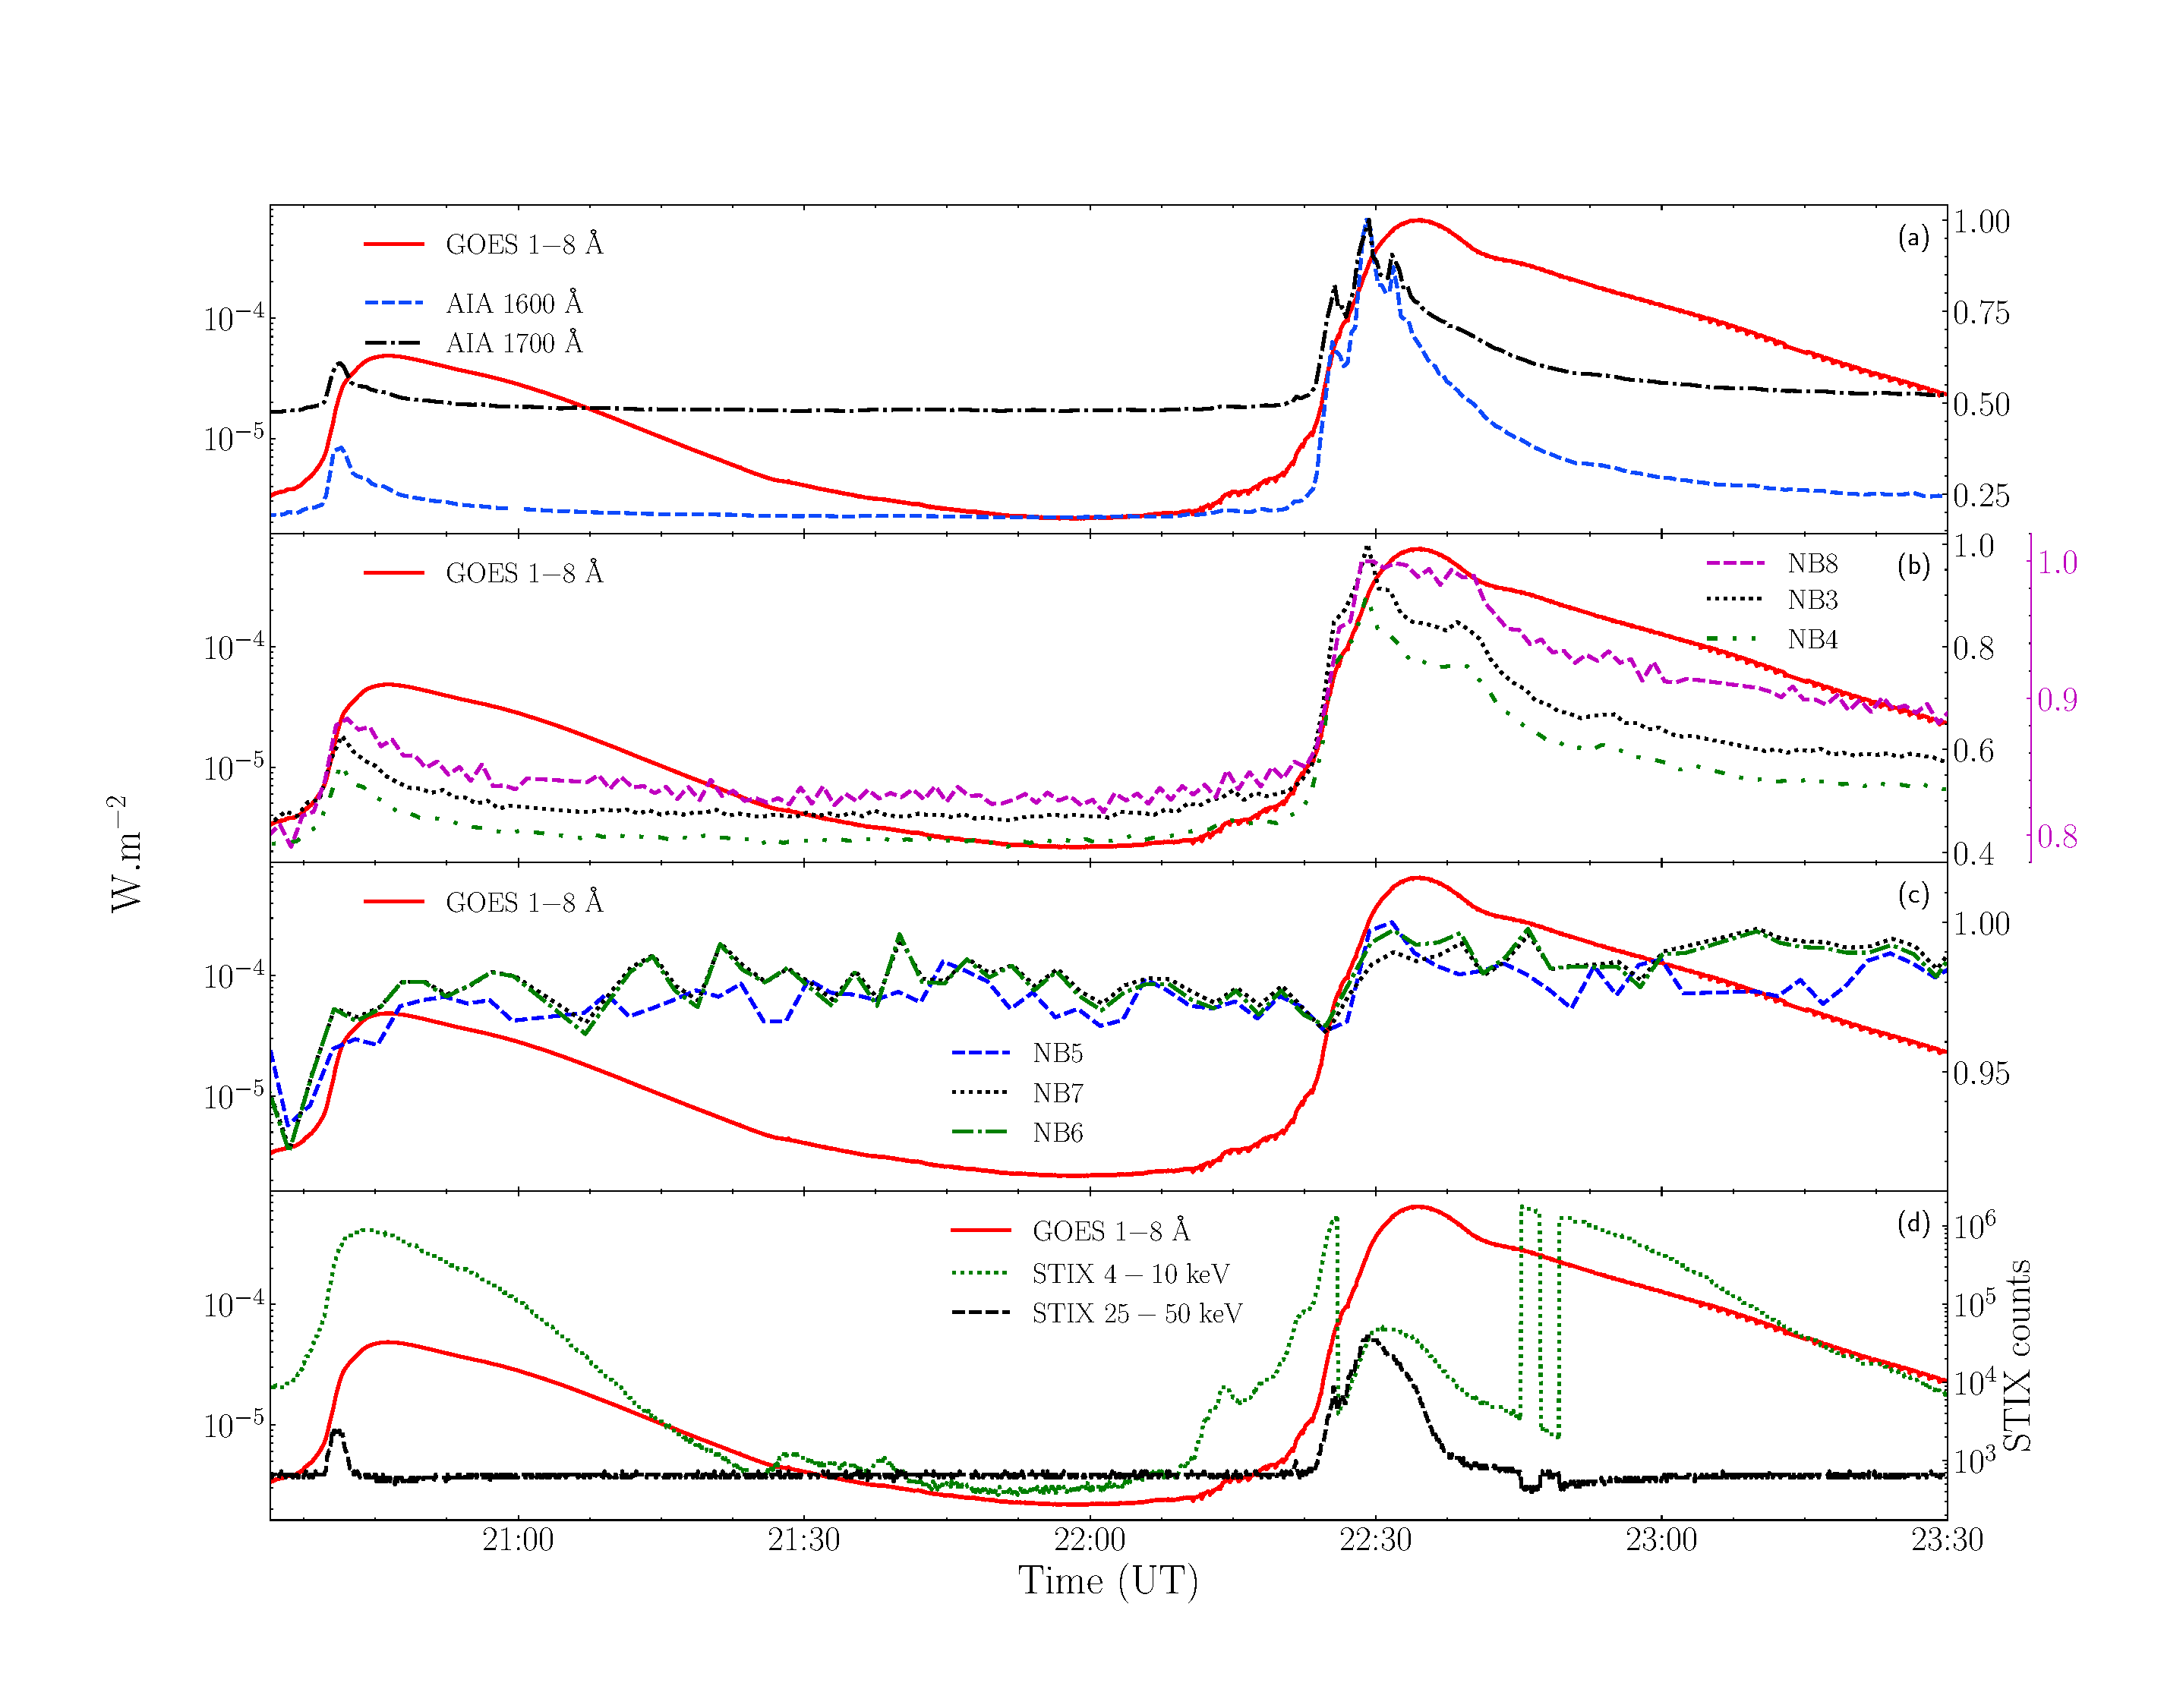
\includegraphics[width=0.8\textwidth,trim={2.3cm 2.5cm 1cm 4.5cm},clip]{lc_full_suit_contour.pdf}
    \caption{Light curves from the whole RoI FoV of \suit~observations compared with AIA, {\it GOES} and STIX observation for the two flares.}
    \label{fig:flare_full}
\end{figure}
%%%%%%%%%

The X6.3 flare provides a good example of the response of the local plasma environment to the flare in the Near Ultraviolet (NUV) regime in 200 {--} 400 nm. The flare peaked around $\sim$ 22:34 UT in the {\it GOES} observation. Images from six narrow band (NB) channels of \suit~ are shown in Fig.~\ref{fig:flare_nb3_peak} top panel at around $\sim$ 22:28-22:29 UT. This is at the peak of the NB3 (\ion{Mg}{2} k 279.6 nm) channel, as observed by \suit. The 60\% peak intensity contour of the NB3 intensity is marked with the black line in all figures of Fig.~\ref{fig:flare_nb3_peak} top panel. From the figure, we also see a similar structure in the NB4 (\ion{Mg}{2} h 280.3 nm) and NB8 (\ion{Ca}{2} h 396.9 nm). No similar structure is observed in the other continuum channels of Fig.~\ref{fig:flare_nb3_peak} top panel.

In Fig.~\ref{fig:flare_nb3_peak} bottom panel, we show the flare observations by \suit~ at their respective peaks. Again, we see very similar structures in NB3, NB4, and NB8. NB3 and NB4 peak at almost the same time $\sim$ 22:29 UT. Although NB8 shows a similar structure, the peak intensity of NB8 is observed slightly later around $\sim$ 22:29:41 UT. The peak intensities of the other continuum NB channels are observed progressively later. The NB5 (Red wing of the Mg window) peaks around $\sim$ 22:32:41 UT. Faint signatures of flare brightening are observed in NB5, marked with red arrows in Fig.~\ref{fig:flare_nb3_peak} bottom panel. No such signatures are observed as clearly in NB6 and NB7. Both of these channels peak around $\sim$ 22:28 UT.

%%%%%%%%%
\begin{figure}[ht!]
    \centering
    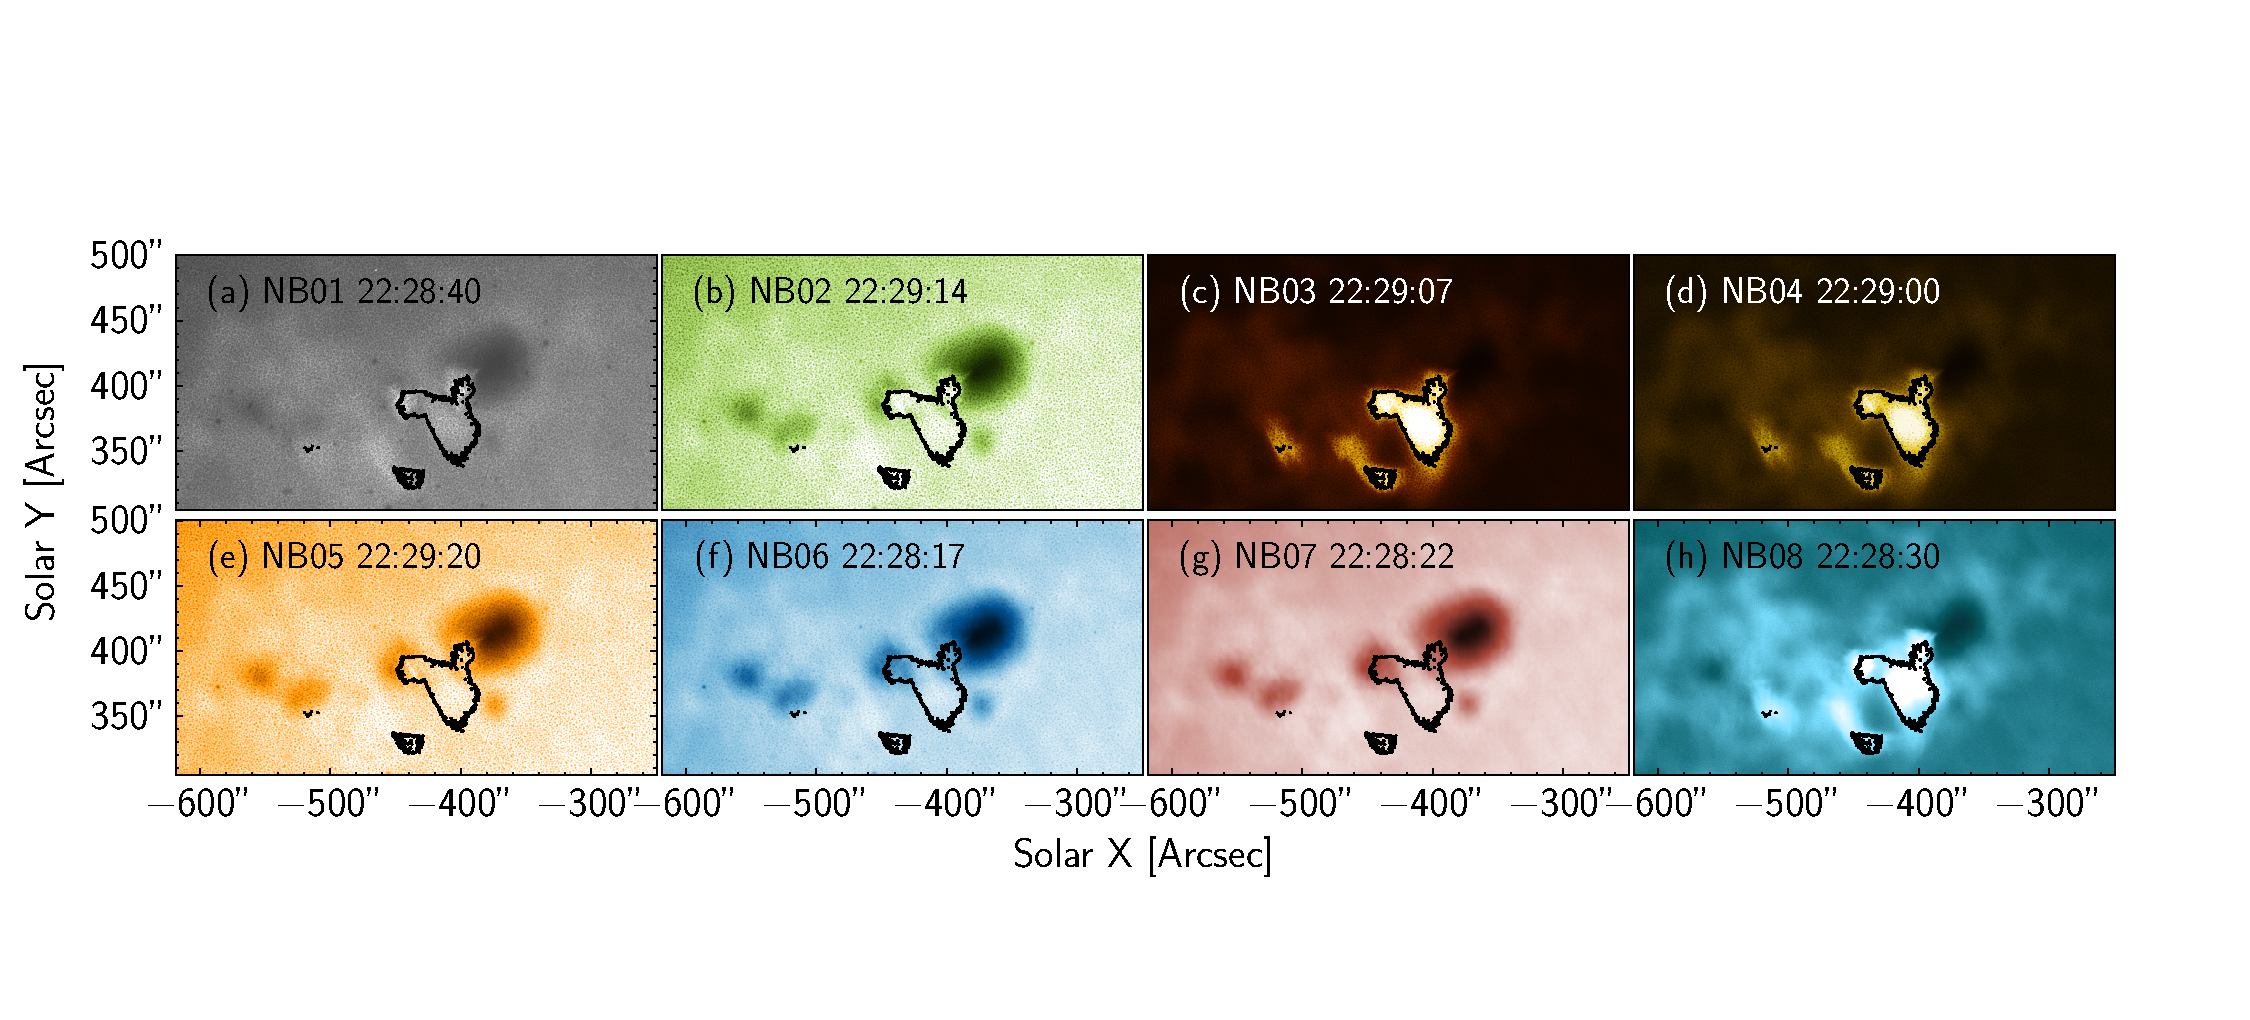
\includegraphics[trim={0cm 0.65cm 0cm 0cm},clip,width=0.5\textwidth]{suit_roi_nb3_peak.pdf} \\
    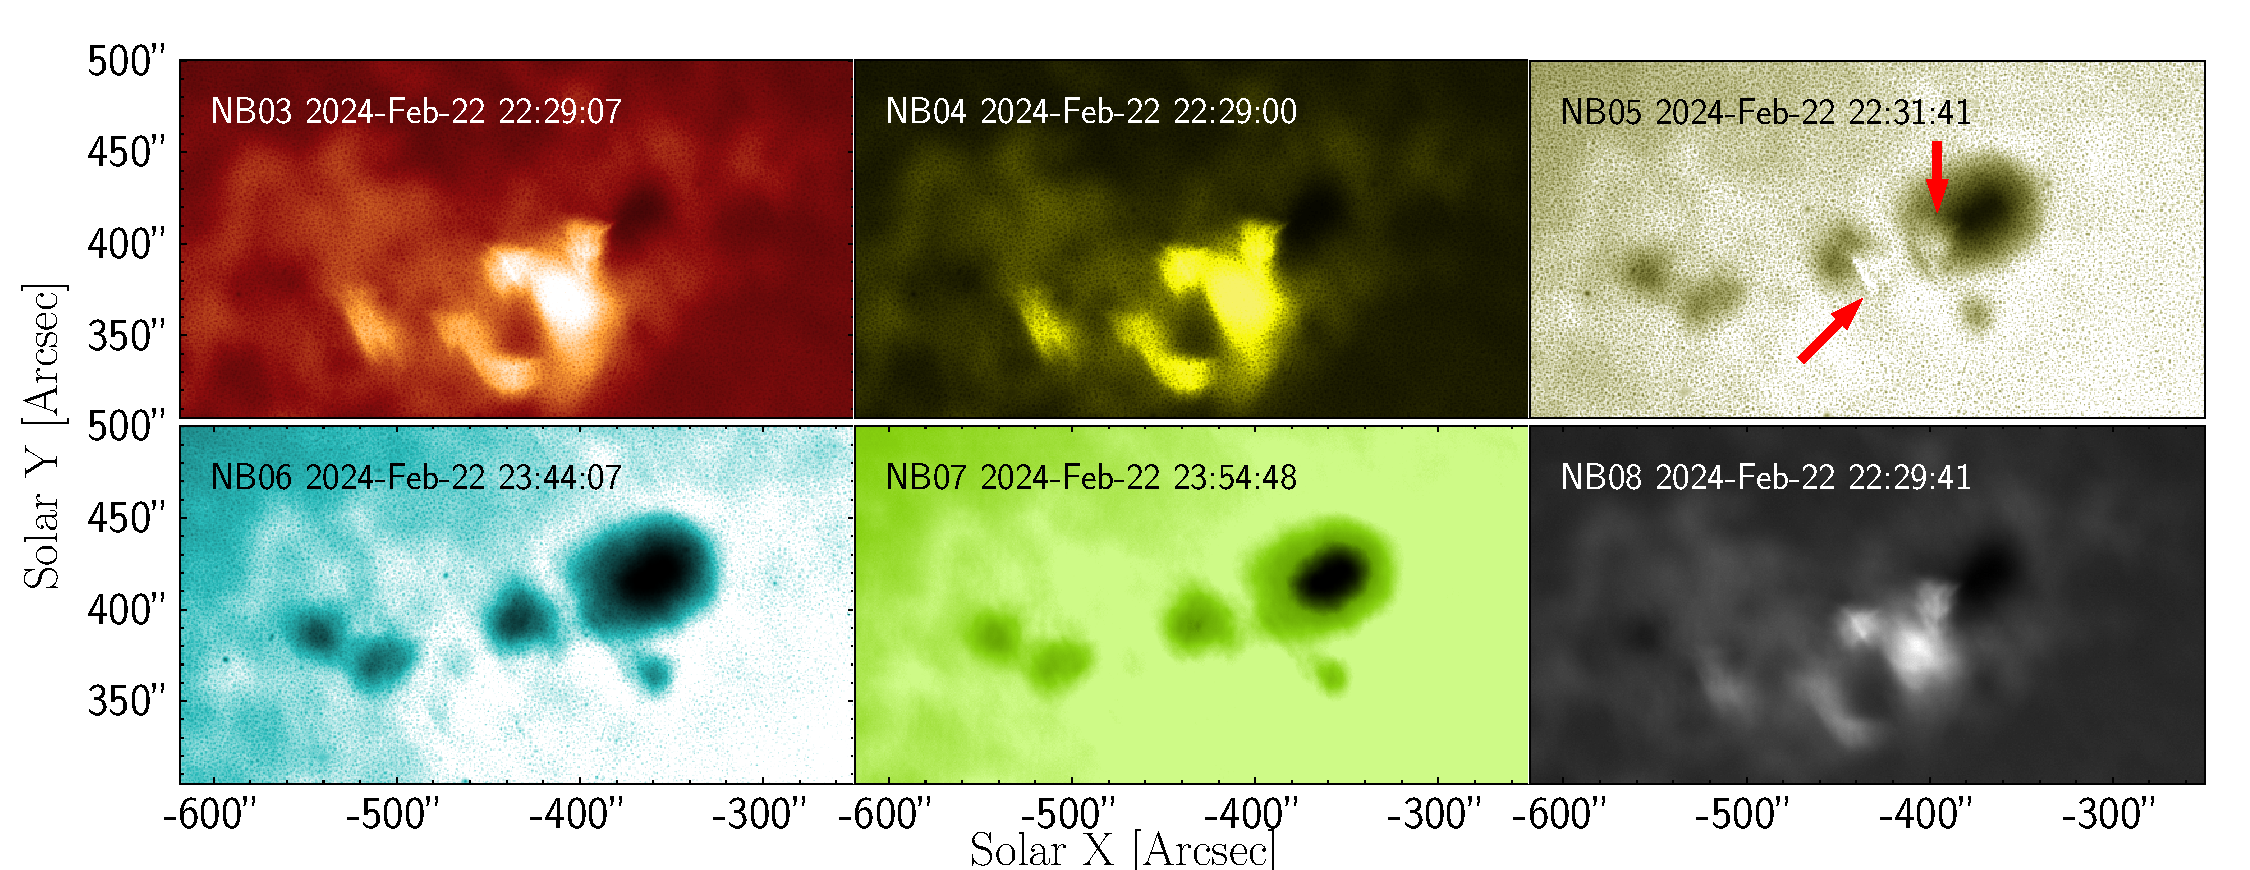
\includegraphics[width=0.5\textwidth]{suit_roi_all_peak.pdf}
    \caption{\suit~observations of the flare from various NB filters. Top panel: during NB3 peak. Bottom panel: During the peak of individual bands.}
    \label{fig:flare_nb3_peak}
\end{figure}
%%%%%%%%%

In Fig.~\ref{fig:flare_lc_suit}, we plot the light curve of the event to compare the observations across various bands. The AIA and \suit~ light curves in Fig.~\ref{fig:flare_lc_suit} are calculated by adding the counts within the region of 60\% peak intensity contour of NB3 (shown in Fig.~\ref{fig:flare_nb3_peak} top panel), after co-aligning and registering the AIA and \suit~observations and normalizing them to the peak intensity. In Fig.~\ref{fig:flare_lc_suit}.a, we show the GOES 1 {--} 8 {\AA} light curve in comparison to AIA 1600 {\AA} and AIA 1700 {\AA}. The AIA 1600 and 1700 {\AA} light curve peaks around $\sim$ 5 minutes earlier than the {\it GOES} peak. 

In Fig.~\ref{fig:flare_lc_suit}.b, we show the GOES 1 {--} 8 {\AA} light curve in comparison to the NB3, NB4 and NB8 light curves. All the NB light curves behave remarkably similarly. The vertical dotted black line across all the panels in Fig.~\ref{fig:flare_lc_suit} denotes the peak intensity in NB3. NB3, NB4, and NB8 peaks around $\sim$ 22:29 UT, which is very similar to AIA 1600 {\AA} and 1700 {\AA}. We also plot the {\it GONG}-H$\alpha$ light curve from the \suit~contour region. The {\it GONG} light curve also peaks at around $\sim$ 22:29 UT. Both NB8 and {\it GONG}-H$\alpha$ shows less contrast variation in the light curve than NB3 and NB4.

We show the GOES 1 {--} 8 {\AA} light curve in comparison to the NB5 (Red wing of the Mg lines, blue dashed), NB6 and NB7 continuum channels in Fig.~\ref{fig:flare_lc_suit}.c. NB5 shows signs of flare response, although much weaker than NB3, NB4 and NB8. NB5 peaks around $\sim$ 22:31 UT, about $\sim$ 3 minutes later than NB3. Similar traits were observed from the images also, as pointed out in Fig.~\ref{fig:flare_nb3_peak} bottom panel and the accompanying discussions. More interestingly, NB6 and NB7 do not show the hallmark sign of a flare light curve, i.e. gradual increase and decrease in the intensity. These bands exhibit a slow but steady rise in intensity after the flare. Finally, in Fig.~\ref{fig:flare_lc_suit}.d, we show the {\it GOES} 1 {--} 8 {\AA} light curve in comparison to the STIX hard and soft X-ray light curve. The hard X-ray peaks around a similar time around $\sim$ 22:29 UT, similar to NB3, NB4 and AIA 1600 and 1700 {\AA}.

%%%%%%%%%
\begin{figure}[ht!]
    \centering
    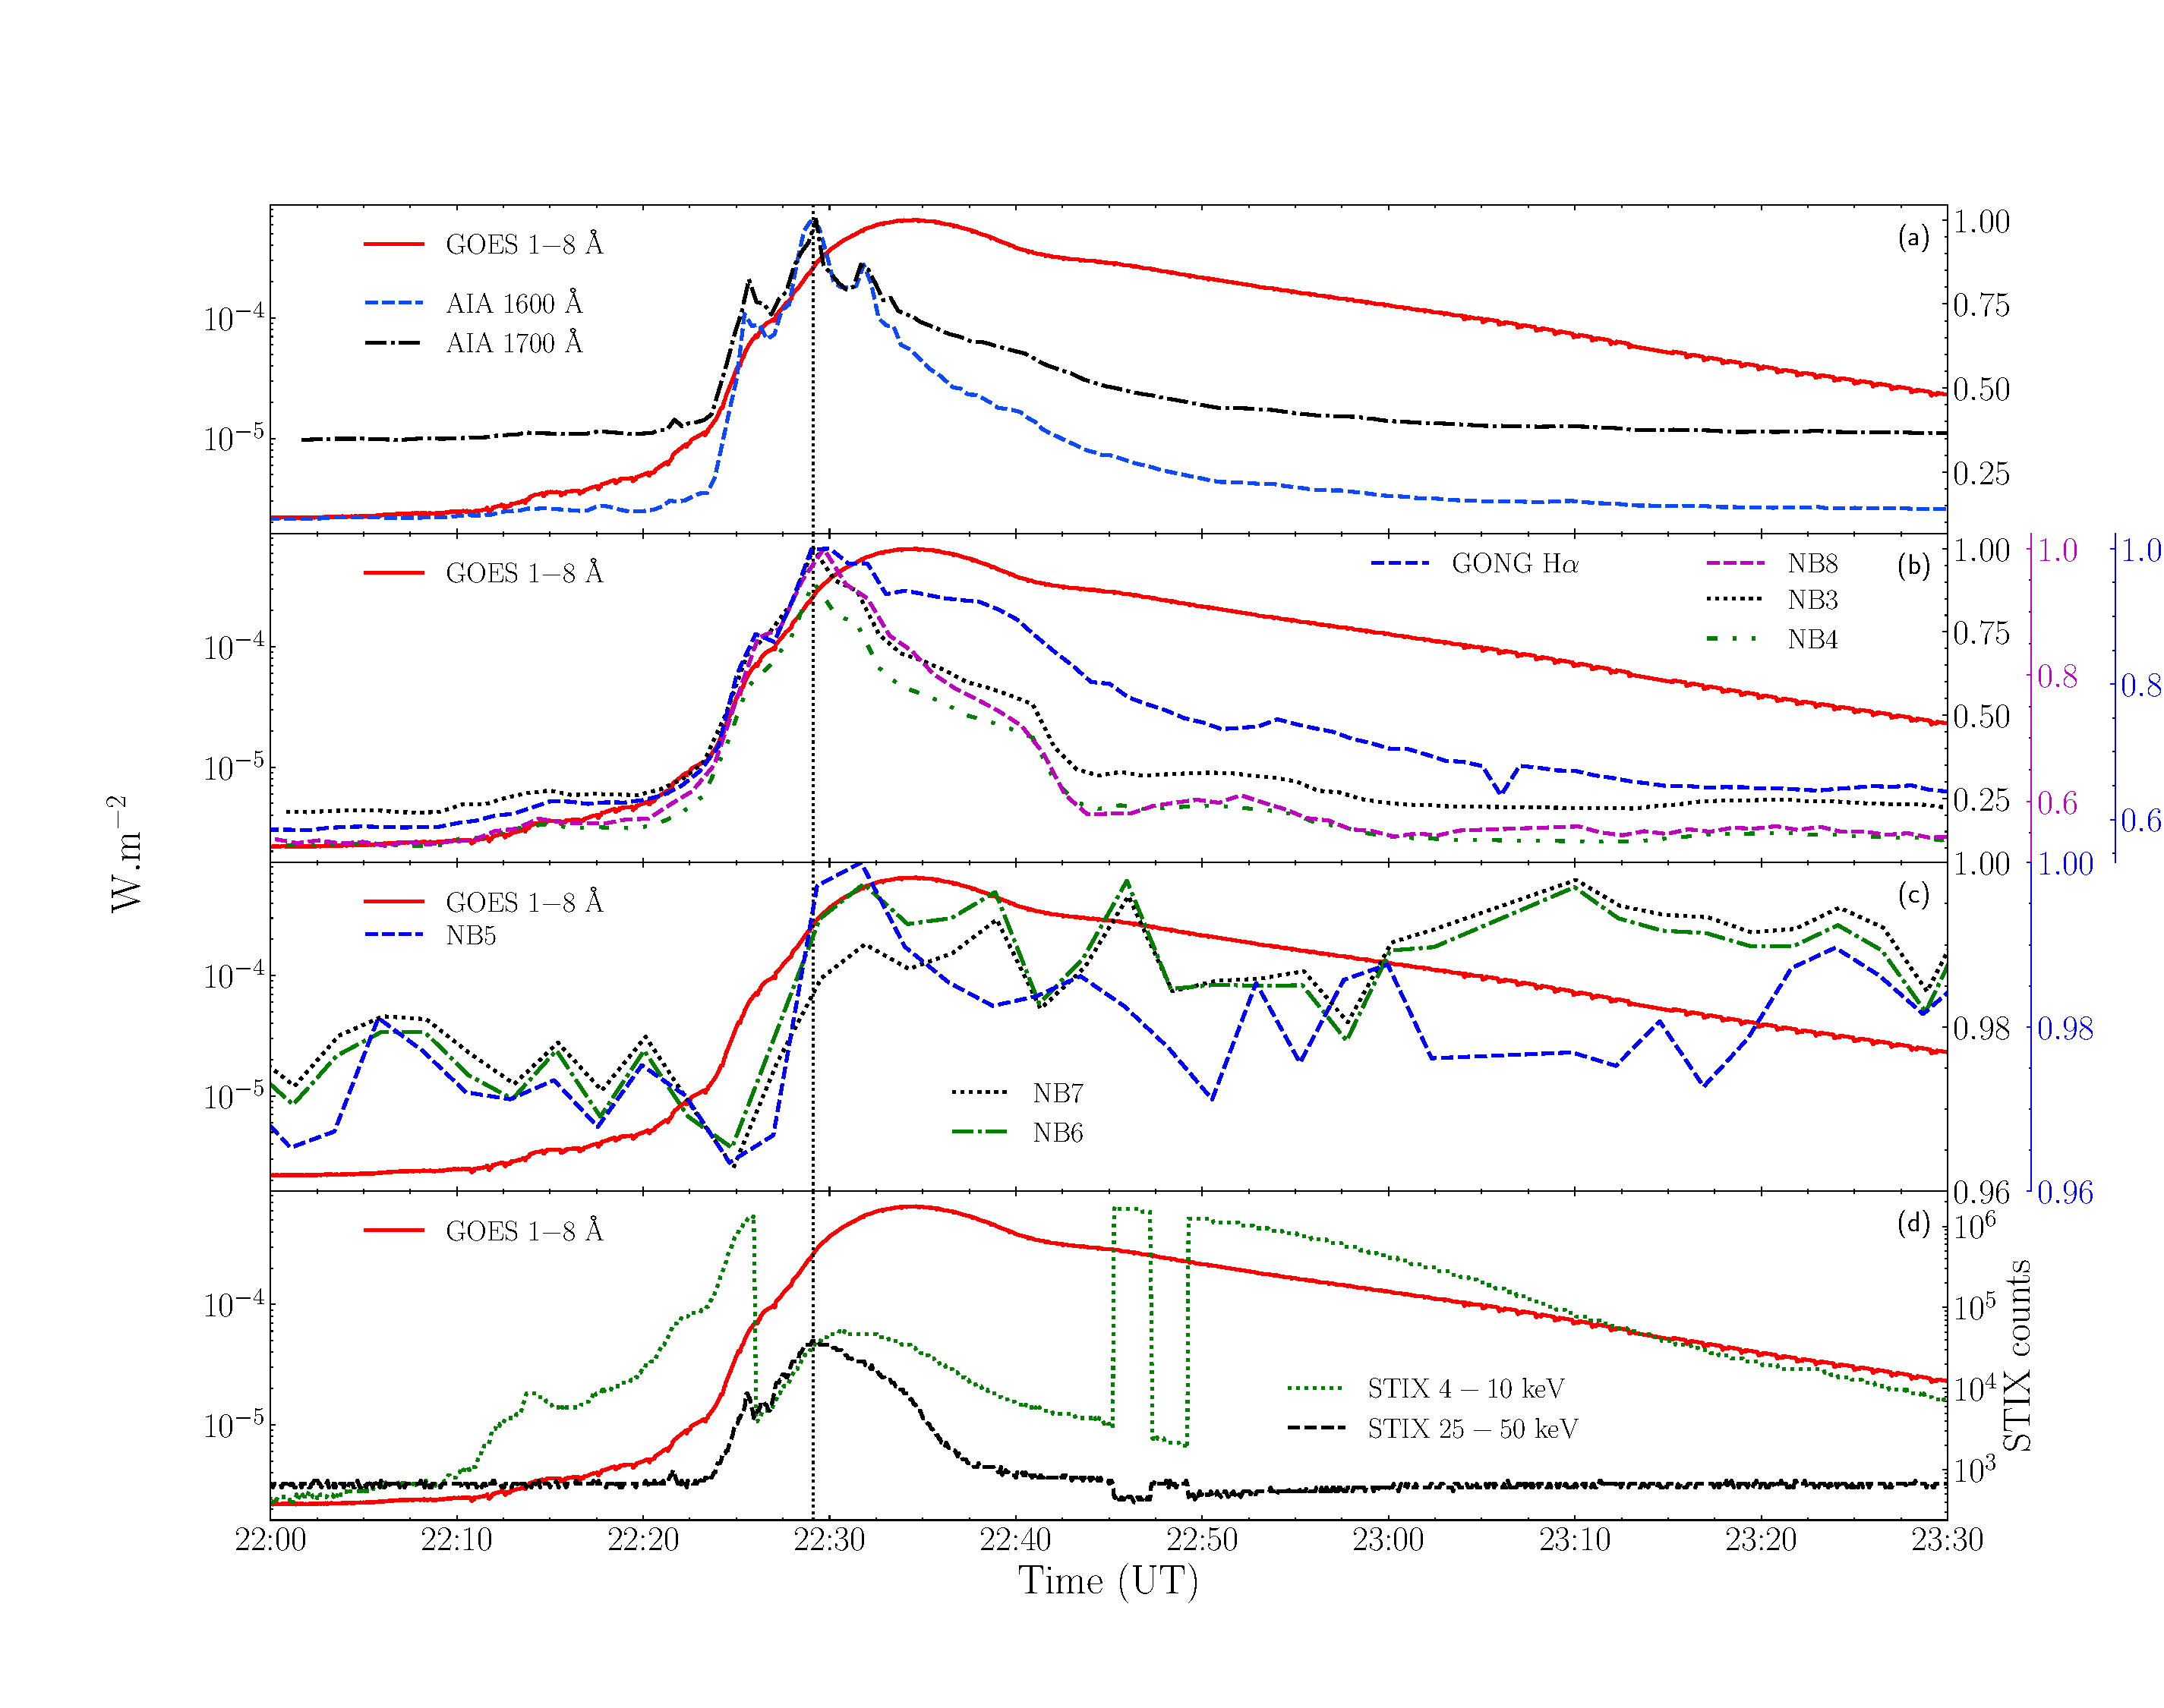
\includegraphics[width=0.8\textwidth,trim={2.3cm 2.5cm 0cm 4.5cm},clip]{lc_suit_contour.pdf}
    \caption{Light curves from the pixels within intensity contour picked from \suit~and co-aligned AIA observations. The NB4 light curve in the second panel is offset by -0.1 from NB3 for better visibility. The vertical dotted dark line marks the flare's peak in NB3 observation.}
    \label{fig:flare_lc_suit}
\end{figure}
%%%%%%%%%

%%%%%%% ############# %%%%%%%
\subsection{XSM-spectra}\label{sec:xsm}
%%%%%%% ############# %%%%%%%

The Solar X-ray monitor on {\it Chandrayan-2}\citep[{\it Chandrayan-2}/XSM,][]{xsm} provides sun as a star soft X-ray spectra in 1{--}15 keV with 1s cadence and significantly better spectral resolution (180 eV at 5.9 keV) compared to STIX (1 keV ar 5.9 keV). The high spectral and temporal resolution allows us to measure the change in elemental abundances over the duration of the flares. XSM observed both flares with coverage in both impulsive and decay phase. The existing studies with XSM has successfully studies the thermal and elemental abundance evolution of various flares \citep{mondal21,kkepa23,nama23}.

Both the M and X-class flares were observed by XSM. The XSM 1{--}8 {\AA} light curves are plotted in Fig.~\ref{fig:xsm-obs} top panel. The red shaded region marks the time window where the Be filter was inserted to prevent saturation. There are periodic gaps in the data due to periodic lunar occultation. We show the spectra obtained by XSM in Fig.~\ref{fig:xsm-obs} bottom panel, during various phases of the flare. The violet spectra at 22:33 UT is near the flare peak, and shows a sharp decrease below 3 keV due to the insertion of the Be filter to avoid saturation. Various Mg, Al, S and Si lines are visible in the pre-flare spectra. In stark contrast during impulsive and peak of the flare we see strong signatures of Ca, Ar and Fe. Due to the uncertainty of the spectra during the Be window observation in $<~3~\mathrm{keV}$ regime, we fit the spectra beyond 3 keV throughput this analysis. We fit the spectra with the XSPEC model {\it chisoth}, which uses a wide range of pre-calculated spectra to fit the observed spectra (For more details please refer to the appendix of \cite{mondal21}).

%%%%%%%%
\begin{figure}[ht!]
\centering
    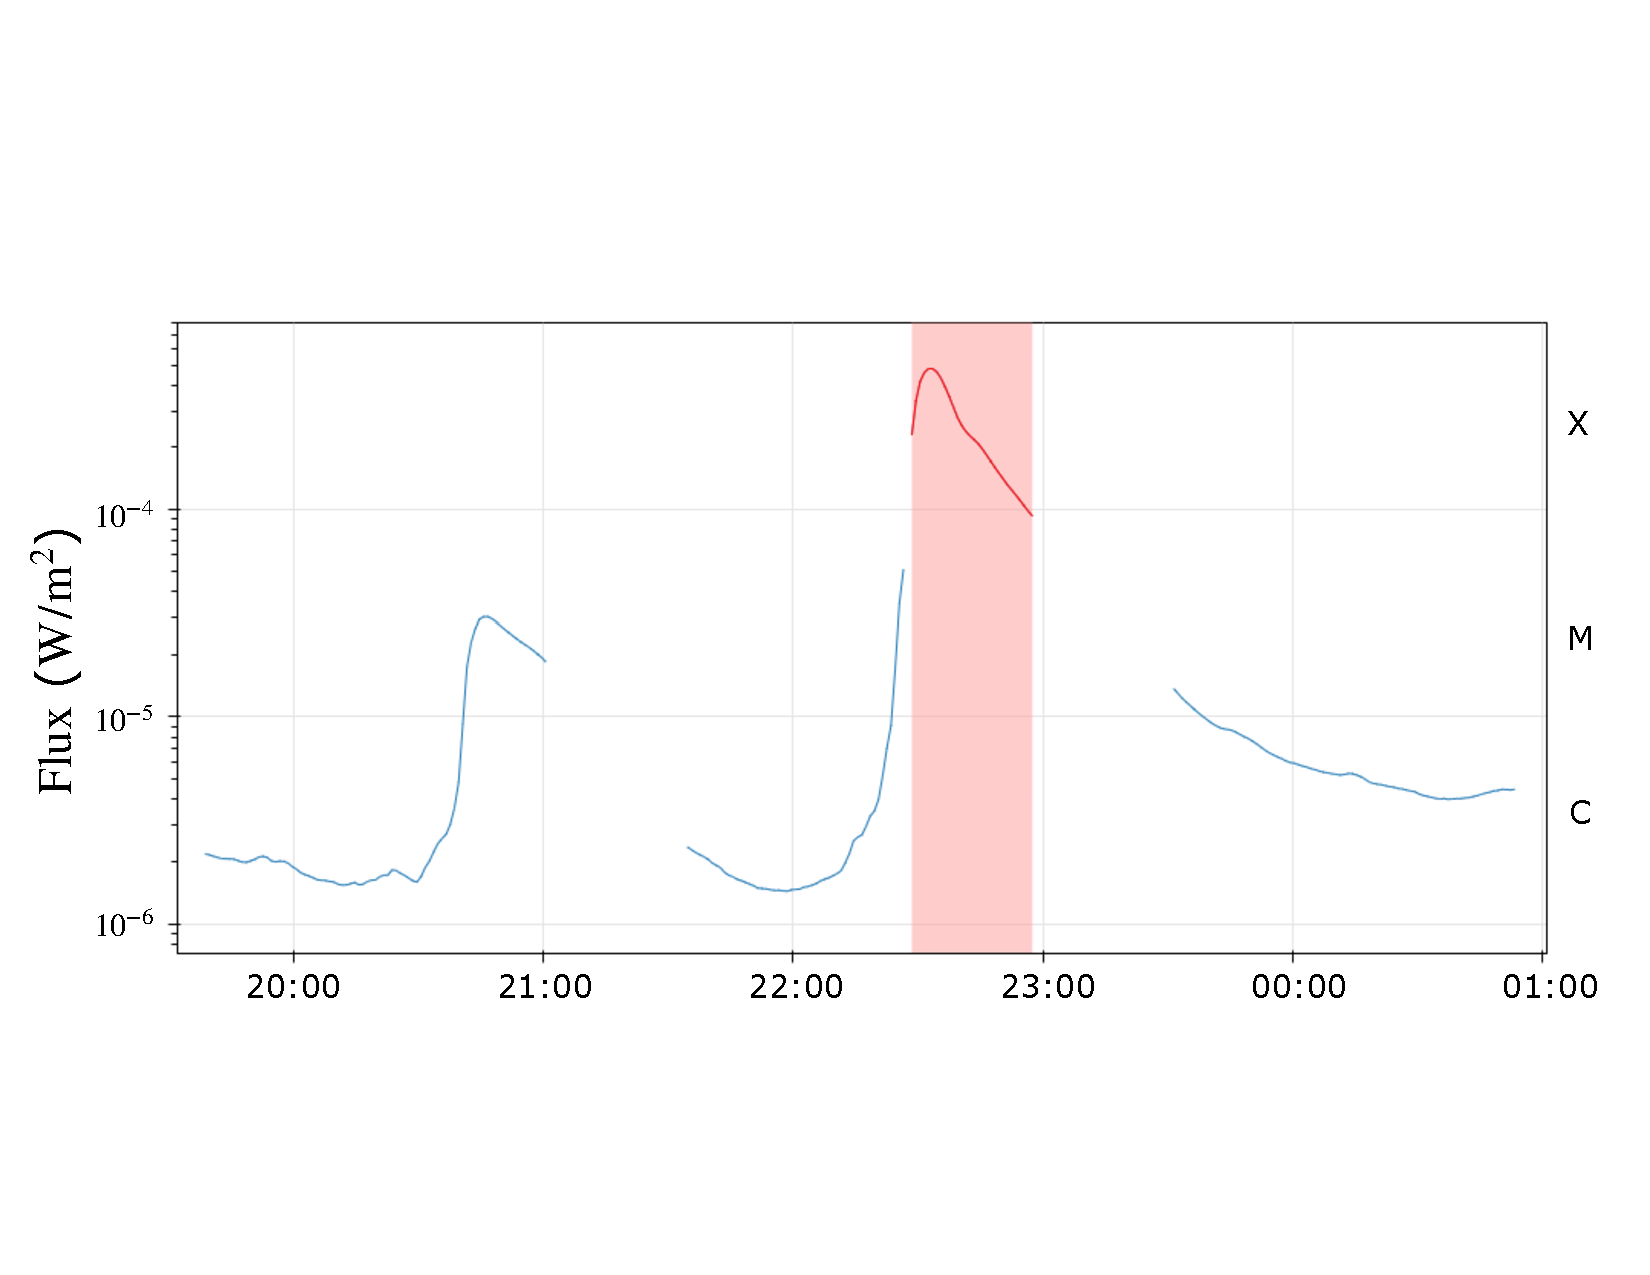
\includegraphics[trim={0.5cm 3.3cm 0.8cm 4cm}, clip, width=0.76\textwidth]{xsm_lc.pdf} \\
    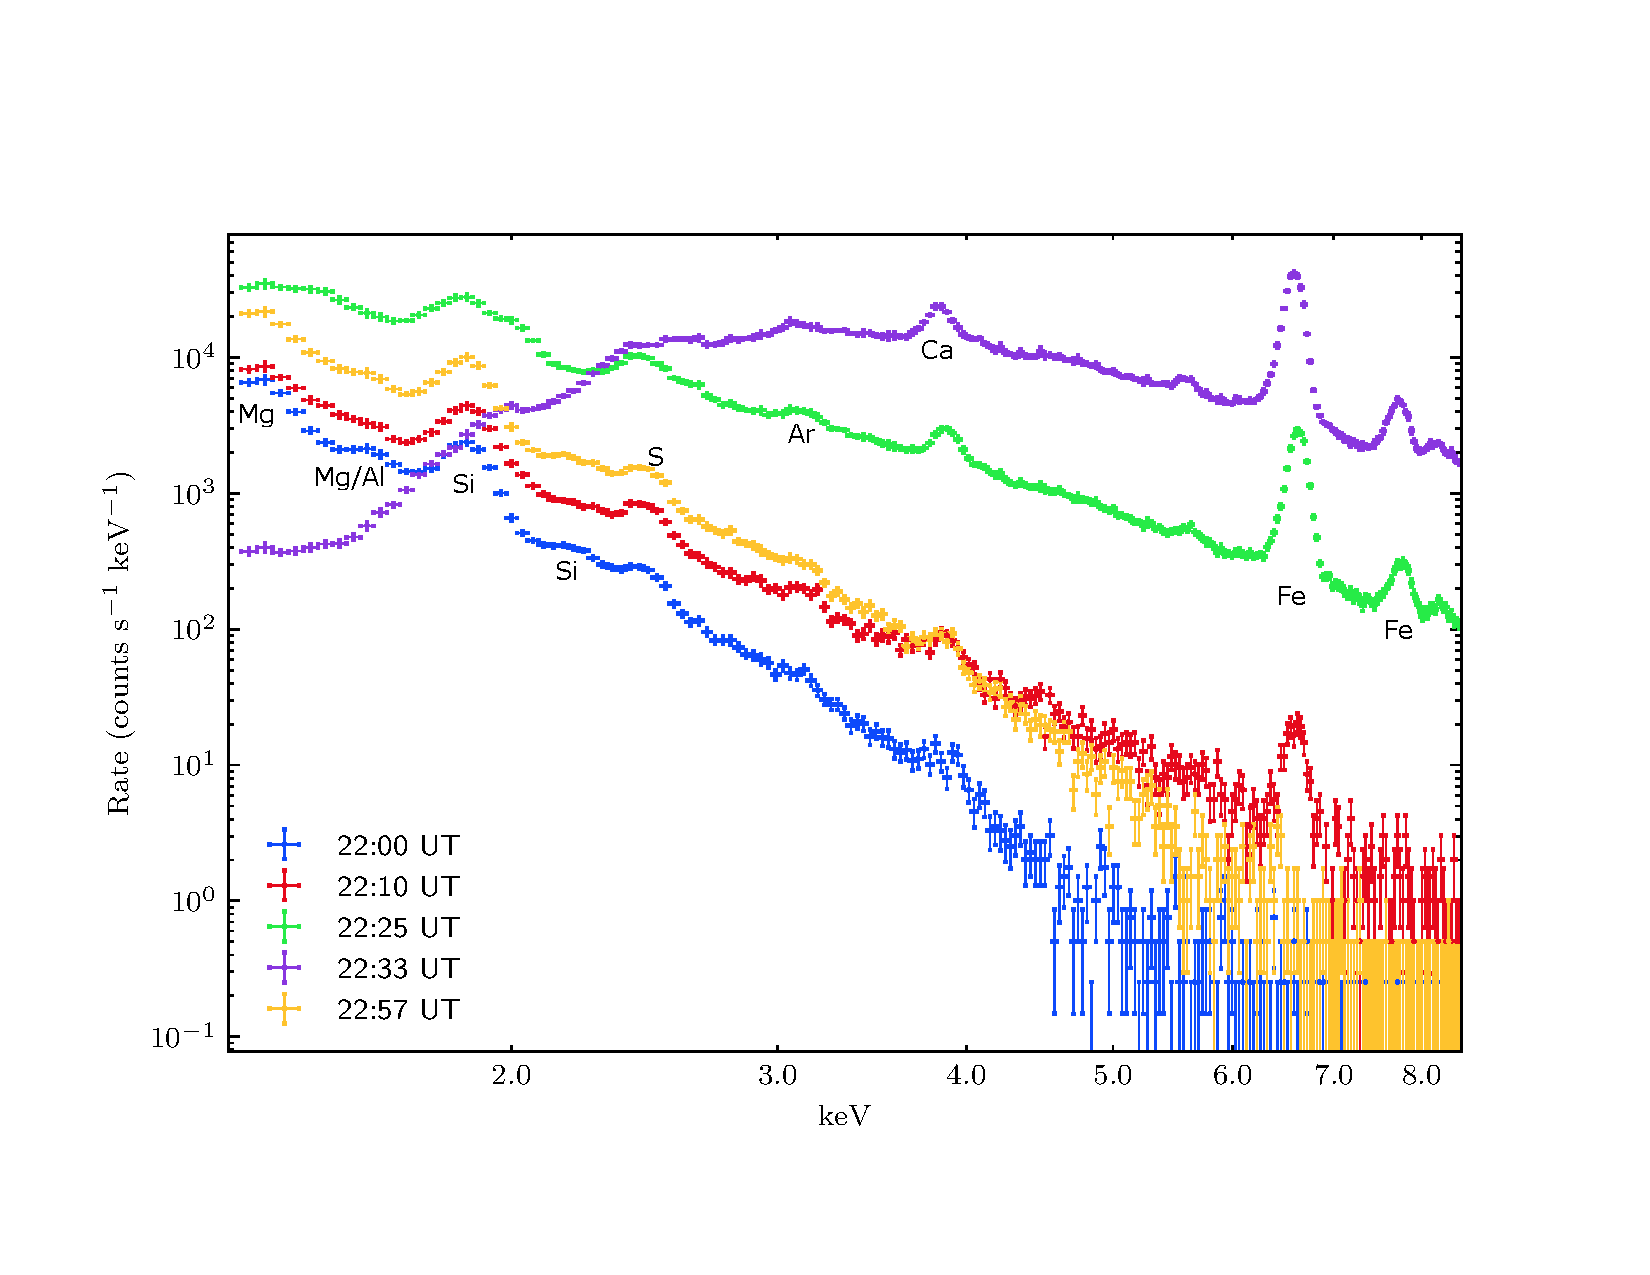
\includegraphics[trim={1.8cm 2.5cm 3cm 3cm},clip,width=0.75\textwidth]{xsm_spec.pdf}
    \caption{Top panel: XSM observation of the two flares. The red shaded region marks the window when the Be filter was inserted. Bottom panel: X-ray spectra during various phases of the flare. The violet spectra is during the soft X-ray peak of the flare and shows a sharp decrease in the intensity below 3 keV. This is due to the insertion of Be filter to avoid saturation.}
    \label{fig:xsm-obs}
\end{figure}
%%%%%%%%

%%%%%%% ############# %%%%%%%
\subsubsection{Fitting XSM spectra}\label{sec:xsm-fit}
%%%%%%% ############# %%%%%%%

The observed soft X-ray spectra from the flaring plasma can be modelled by an isothermal plasma characterized by various parameters {\it e.g.} temperature, emission measure and abundance of various elements. As alluded earlier, we use the `{\it chisoth}' model \citep{mondal21} to fit the observed spectra from XSM. The `{\it chisoth}' model uses CHIANTI atomic database \cite{chianti} to calculate spectra for individual elements over a large temperature grid and stores as tables. The model includes elements from H (Z=1) to Zn (Z=30). The spectra of individual elements are calculated over a wide temperature range (0.3 {--} 50 MK). These modelled spectra of various elemental abundance over a wide temperature range are loaded in XSPEC and added with varying weights to fit the observed spectra. The Total model spectrum is given by  $$I_{mod}(T)~=~EM\sum_{X}I_{X}(T)N_{X}$$`EM' is the volume emission measure, $N_{X}$ is the abundance of element X relative to H and $I_{X}(T)$ is the modelled spectrum of element X at temperature T. The fit is done in a recursive process by minimizing the chi-squared between the observed and modelled spectra.

We initially used an isothermal model to fit the spectra. One of the key observations we make is a presence of systematic residual around the Fe complex around $\sim$ 6.5 keV. This is illustrated in the top panel of Fig.~\ref{fig:xsm_fit} top panel, where there is an excess visible in the blue side of the Fe line complex at $\sim$ 6.7 keV. \cite{mithun22} could not explain this systematic excess with multithermal DEM distributions. One of the possible explanation of this excess flux is Fe fluorescence emission. There have been observations of Fe line fluorescence at 6.4 keV (Fe K$\alpha$) and 7.06 keV (Fe K$\beta$) \citep{neupert67,doscheck71,bai79,tanaka84,parmar84,phillips12} using high-resolution X-ray spectra from Bent Crystal Spectrometer on-board Solar Maximum Mission \citep[Bent/{\it SMM},][]{bent,smm} and Yokoh \citep{yokoh} mission. Previous studies have suggested that this emission arises from the excitation of low ionization state Fe in the Photosphere either via the X-ray from the flaring plasma \citep{bai79} or directly from the non-thermal electron beam \citep{phillips73}. The Fe K$\alpha$ fluorescence is usually dependent on the position on the solar disk \citep{parmar84}. The emergent Fe K$\alpha$ emission suffers significant absorption and scattering along the line of sight, which increases with increasing heliocentric angle, resulting in a decrease in the observed intensity. For our event, the flaring region is near the disk center making the Fe K$\alpha$ fluorescence a valid candidate for explaining the excess. We added a Gaussian component to the `{\it chisoth}' model to get better fit (see Fig.~\ref{fig:flare_obs} bottom panel).

We add a Gaussian line component to our fit at 6.4 keV to explore the possibility of the excess flux arising from Fe K$\alpha$ fluorescence. We find that this fits the observed spectra better than previous instances, as demonstrated in Fig.~\ref{fig:xsm_fit} bottom panel. The K$\alpha$ emission would arise from the X-ray emission from the flaring regions having energies $>$ 7.12 keV, the K edge of Fe, exciting the Fe atoms in the Photosphere. We show the intensity of the fitted Fe 6.4 keV component excess (blue solid line), in comparison to the fitted flux in 7.12 {--} 8.5 keV (green dot-dashed line) in Fig.~\ref{fig:fe_excess} top panel. For reference, {\it GOES} 1{--}8 {\AA} soft X-ray flux (red dotted line) and STIX 25 {--} 50 keV Hard X-ray flux (black dashed line) are overplotted. STIX Hard X-ray is a fair representative of the non-thermal electron flux deposited into the foot points. In the bottom panel, the light curve fitted Fe 6.4 keV excess Gaussian component is plotted with the lightcurve from the bright kernels marked with the two boxes in Fig.~\ref{fig:flare_nb3_peak} bottom panel. In both panels, the peak time of the Fe excess (blue solid line), STIX hard X-ray (black dashed line) and NB5 brightness from box 1 (dotted magenta line) are marked with vertical lines.

%%%%%%%%%%
\begin{figure}[ht!]
    \centering
    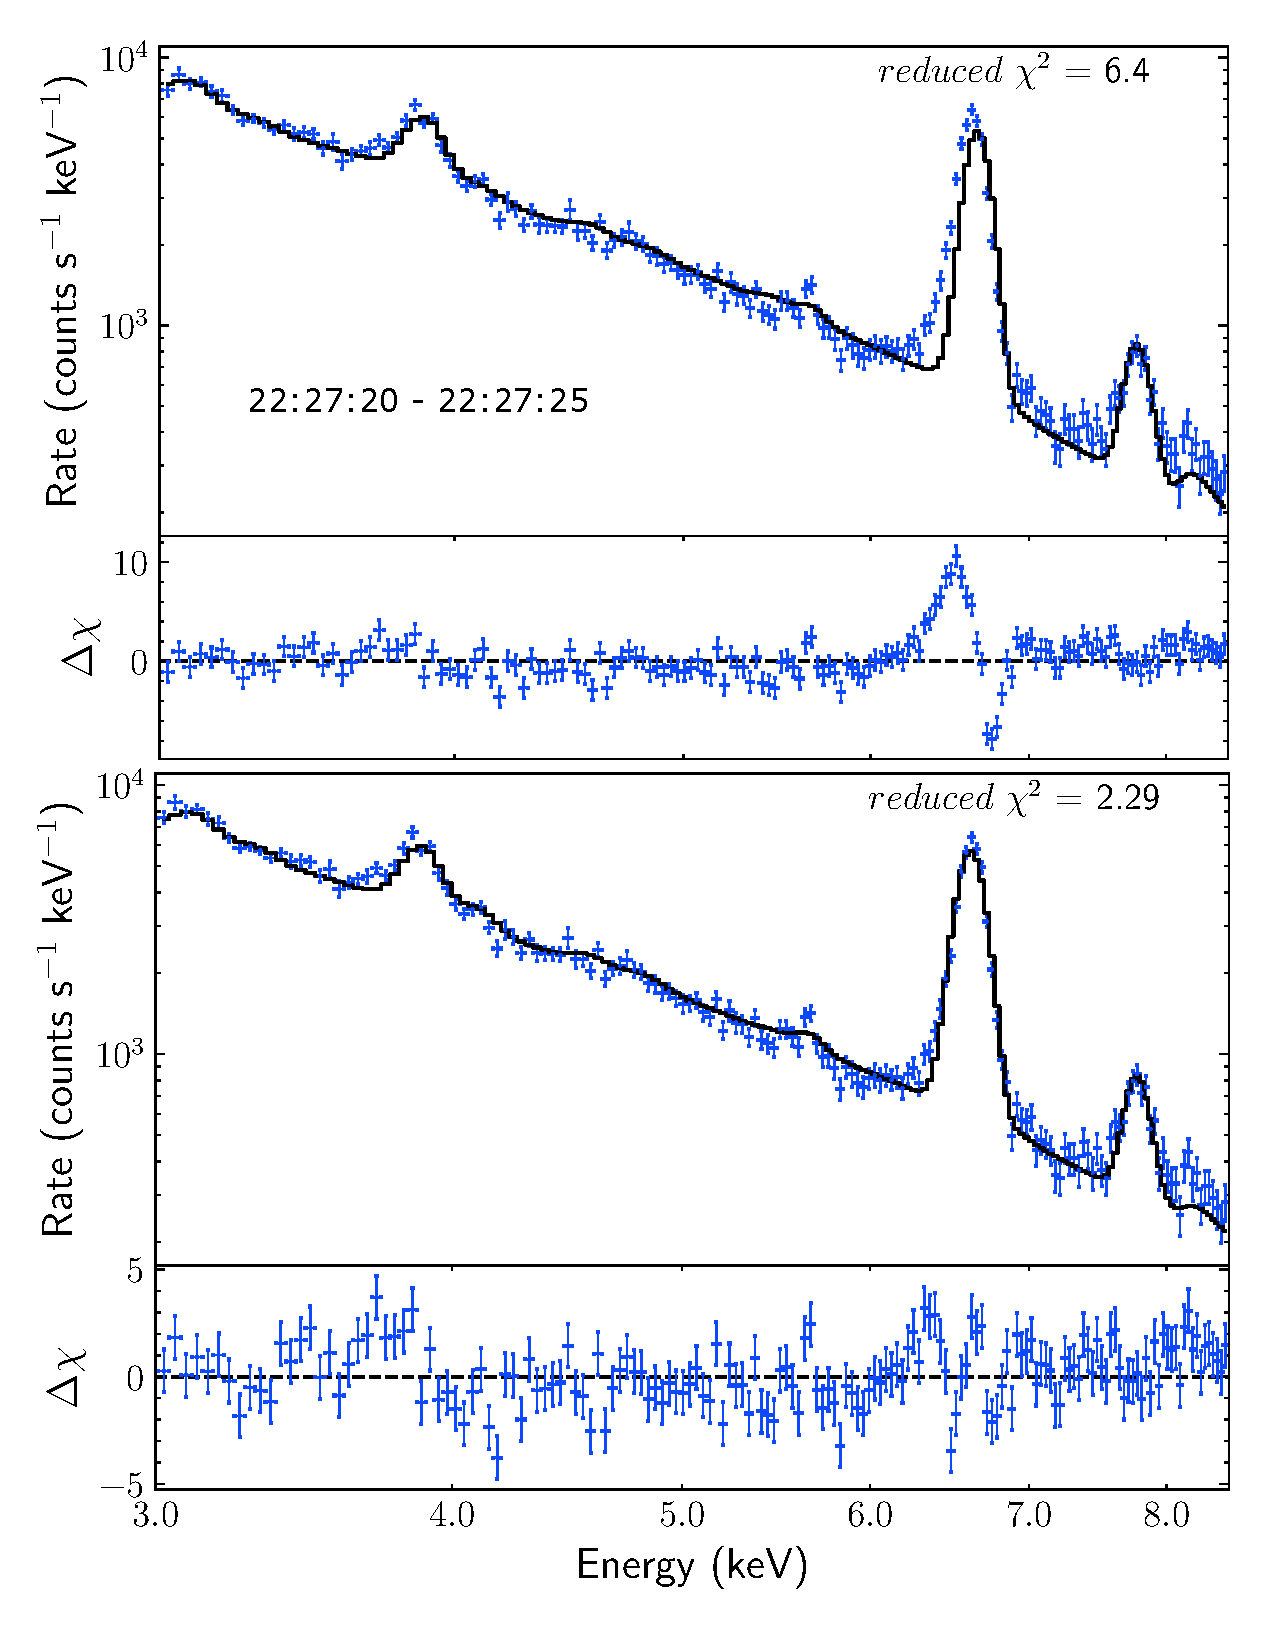
\includegraphics[trim={0.5cm 1cm 0.5cm 0.7cm}, clip, width=0.77\textwidth]{xsm_fit.pdf}
    \caption{XSM spectra in 3 {--} 8.5 keV binned between 22:27:20 {--} 22:27:25 UT. Top panel shows the fit with ``chisoth+chisoth" model. Bottom panel shows the same spectra fitted with ``chisoth+chisoth+gaussian" model.}
    \label{fig:xsm_fit}
\end{figure}
%%%%%%%%%%

%%%%%%%%%%
\begin{figure}[ht!]
\centering
    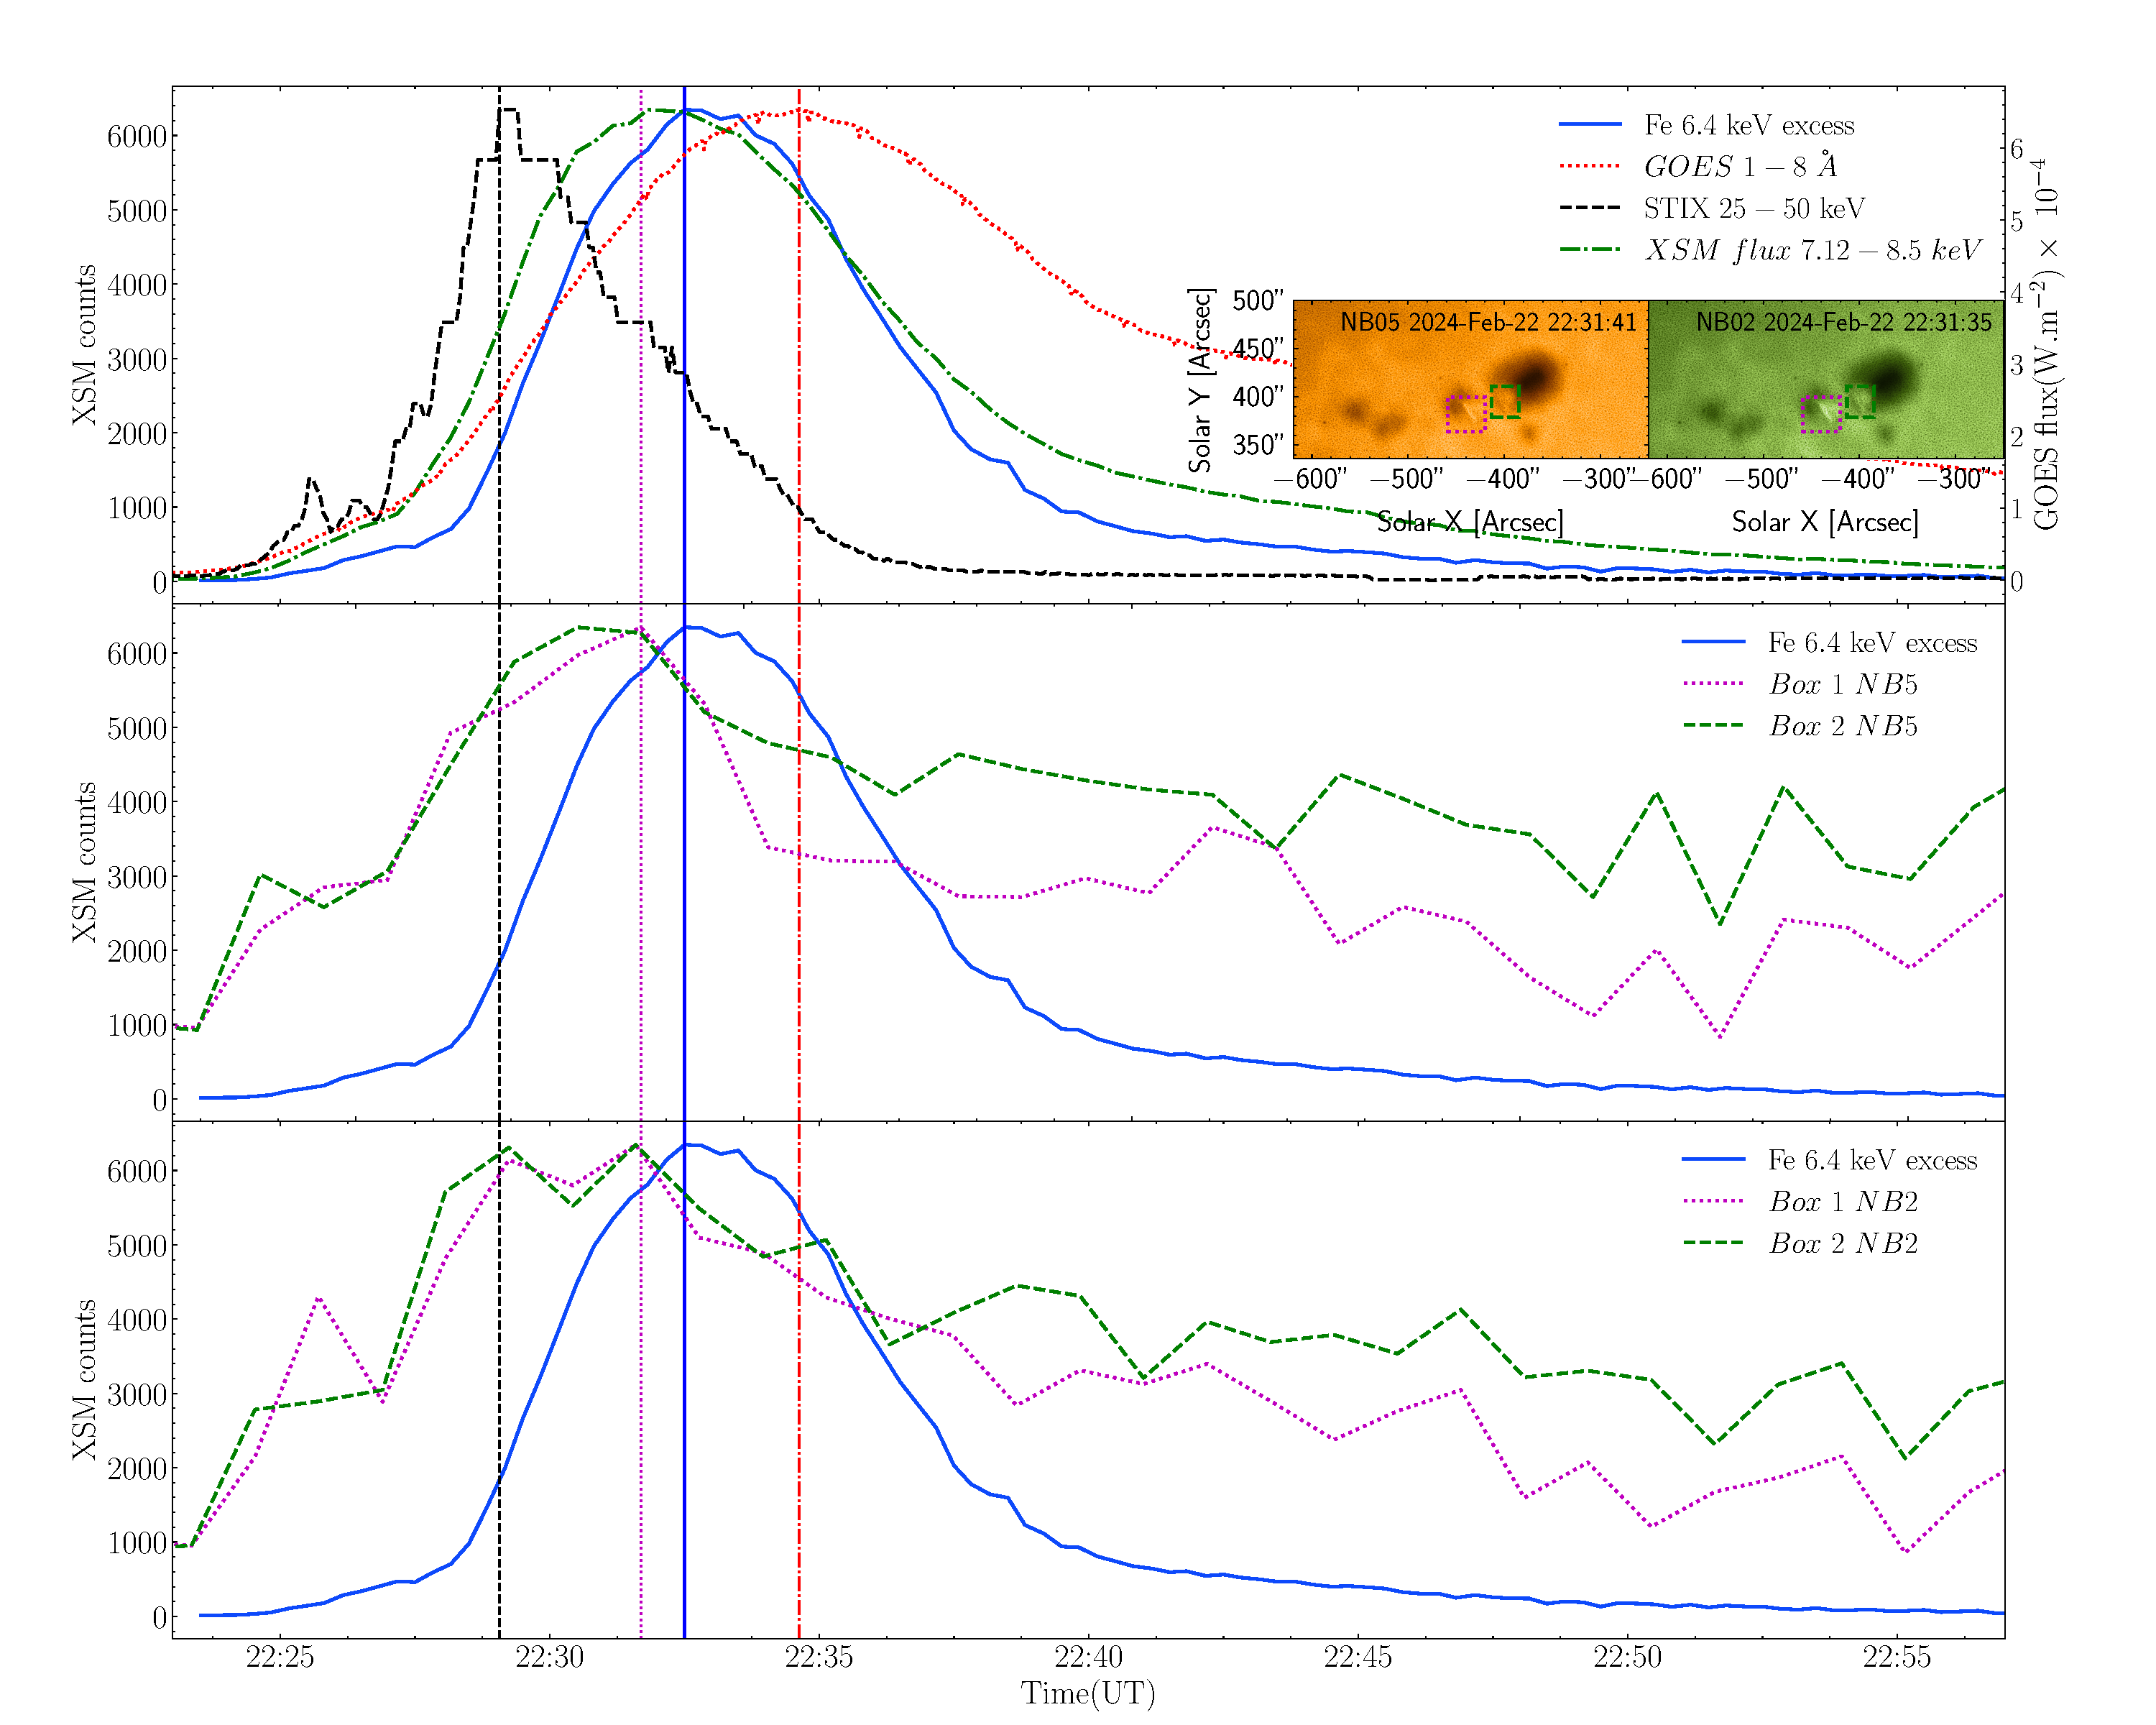
\includegraphics[trim={1.3cm 0.1cm 0.3cm 1.2cm}, clip, width=0.95\textwidth]{fe_excess_4.pdf}
    \caption{Fe excess emission from 6.4 keV(blue solid) in comparison to STIX 25-50 keV(black dashed), GOES 1 {--} 8 $\AA$ (dotted red) and XSM 7.12 {--} 8.5 keV (green dot-dashed) light curve.}
    \label{fig:fe_excess}
\end{figure}
%%%%%%%%%%

%%%%%%% ############# %%%%%%%
\subsection{Discussion}\label{sec:dis1}
%%%%%%% ############# %%%%%%%

This section reports the \suit~narrow band imaging of the first localized flare by the onboard flare detection algorithm. We report the observation in NB3 (\ion{Mg}{2} k 279.6 nm), NB4 (\ion{Mg}{2} h 280.3 nm), NB8 (\ion{Ca}{2} h 396.9 nm) and the continuum channels NB5 (Red wing of \ion{Mg}{2}), NB6 and NB7. For both the flares, the NB3, NB4 and NB8 peak around the same time as AIA 1600 and 1700 {\AA}. For the X6.3 flare, NB3, NB4 behave very similarly to NB8 within the NB3 intensity contour (see Fig.~\ref{fig:flare_lc_suit}.b). But the NB8 peak over the whole active region is much broader compared to the NB3 and NB4 light curves (see Fig.~\ref{fig:flare_full}). This implies that NB8 behaves differently in other parts of the active region.

The NB5 observes the continuum that is usually attributed as the Balmer continuum. There have been previous studies where Photospheric metal lines went into emission and affected the Balmer continuum \citep{heinzel14,kleint17}. The dominant contribution would still be the Balmer continuum. \cite{reetika21} attributed the brightening in the SJI 2832 {\AA} continuum for a mini flare to direct signature of electron beams. \cite{kowalski19} showed for one event, that the SJI 2832 {\AA} continuum enhancement and several Phototspheric absorption lines going into emission can be attributed to significant Photospheric heating. The entire 2832 {\AA} window of IRIS had several \ion{Fe}{2} and \ion{Cr}{2} lines which are usually observed as absorption lines, in emission. Curiously enough, this observation was also made in a bright umbral flare kernel, similar to the current event. As there was no {\it IRIS} scan of the umbral brightening visible in NB5, unfortunately, we can not comment on the spectral nature of the bright kernel.

We see an excess around the 6.5 keV Fe complex from the XSM observations which can be fitted with a single Gaussian. From Fig.~\ref{fig:fe_excess}, the Fe excess light curve (blue solid line) behaves very similar to the soft X-ray flux beyond the Fe K edge at 7.12 keV (green dot-dashed line). The excess also shows no correlation with the STIX 25 {--} 50 keV hard X-ray flux (black dashed line), illustrating no significant contribution from the non-thermal electron flux. This suggests that the excess flux seen around 6.4 keV Fe complex arises from the Fe fluorescence from the flaring X-ray. If we assume the penumbral brightening observed in this flare to be similar as observed by \cite{kowalski19}, the bright kernels observed in NB5 mainly arises from a plethora of \ion{Fe}{2} lines. The flaring X-ray beyond Fe K edge (7.12 keV) photoionizes the Fe in the Photosphere, giving rise to both \ion{Fe}{2} lines in the red wing of \ion{Mg}{2}, along with the observed Fe fluorescence by XSM. 

We see a similar brightening in NB2, the blue wing of the Mg window. The light curve of the brightening of the blue wing of Mg is shown in Fig.~\ref{fig:fe_excess} third panel. The light curve shows peak at both hard X-ray peak and later on closer to Fe excess component peak. This possibly shows both Photospheric and Chromospheric components from the NB2. Further investigation and modelling is required to comment on the local plasma parameters that would produce the bright kernels observed in both NB5 and NB2, with the relative timing within themselves and also in comparison to the various energies in X-ray.

The other interesting observation is the rise in the continuum intensity, specifically in NB6 and NB7 as the flares happen. We can see a steady rise in the continuum intensity after the M and X class flare (see Fig.~\ref{fig:flare_full}). For the X6.3 flare, we do see some signature of the flare in NB5, although it peaks about $\sim$ 5 minutes later compared to NB3 and NB4. The photospheric nature of the NB5 continuum explains the 5-minute delay of the peak from NB3. We see the flare peak in sequential order of formation height NB3 and NB4 (\ion{Mg}{2}, 22:29 UT) and NB8 (\ion{Ca}{2}) $\Longrightarrow$ NB5 (Photospheric continuum, 22:32:41 UT). We are observing the increase in continuum intensity from 283.2 nm to 388 nm. The consistent increase in continuum intensity is happening across the Balmer jump ($\lambda$~=~364.5 nm).

%%----------------------------------------------------
\section{X5 flare observed on Dec 31st, 2023} \label{sec:dec_31st}
%%----------------------------------------------------

NOAA AR 13536 started to appear on the northeast limb on 31st December 2023. It erupted an X5 flare at 21:36 UT. {\suit} was still in the cruise phase, on its way to the L1. The standard synoptic observation mode was not turned on, and {\suit} was only observed in its NB4 (\ion{Mg}{2} h) channel with a minute cadence. AIA, STIX, and SUVI also observed the flare among many other imaging observatories. The {\it GOES} Soft X-ray (SXR) peaked $\sim$ 21:55 UT. The event was located at the heliographic position of $\sim$ [-968{\arcsec}, 88{\arcsec}].

We use JPL horizons system to get the accurate location of the Aditya-L1 spacecraft. We use this location to account for the differences in plate scale between AIA and {\suit} observations. We then co-register and co-align AIA 1600 {\AA} and {\suit} NB4 observations. It is noteworthy that the {\suit} had $\sim$ 7{\degree} roll with respect to AIA during the cruise phase, which needs to be rotated before co-registering the AIA and {\suit} observations. We show a sequence of co-aligned observations in Fig.~\ref{fig:dec_flare_obs}. The AIA 1600 {\AA} observations are plotted in green-black colormap and the {\suit} NB4 observations are plotted in yellow. We see the rising loop in AIA 1600 {\AA} at 21:39 UT. In subsequent frames, we see the ejected plasma blob from NB4 observations is cospatial with the ejected material in AIA 1600 {\AA}.

%%%%%%%%%%
\begin{figure*}[ht!]
    \centering
    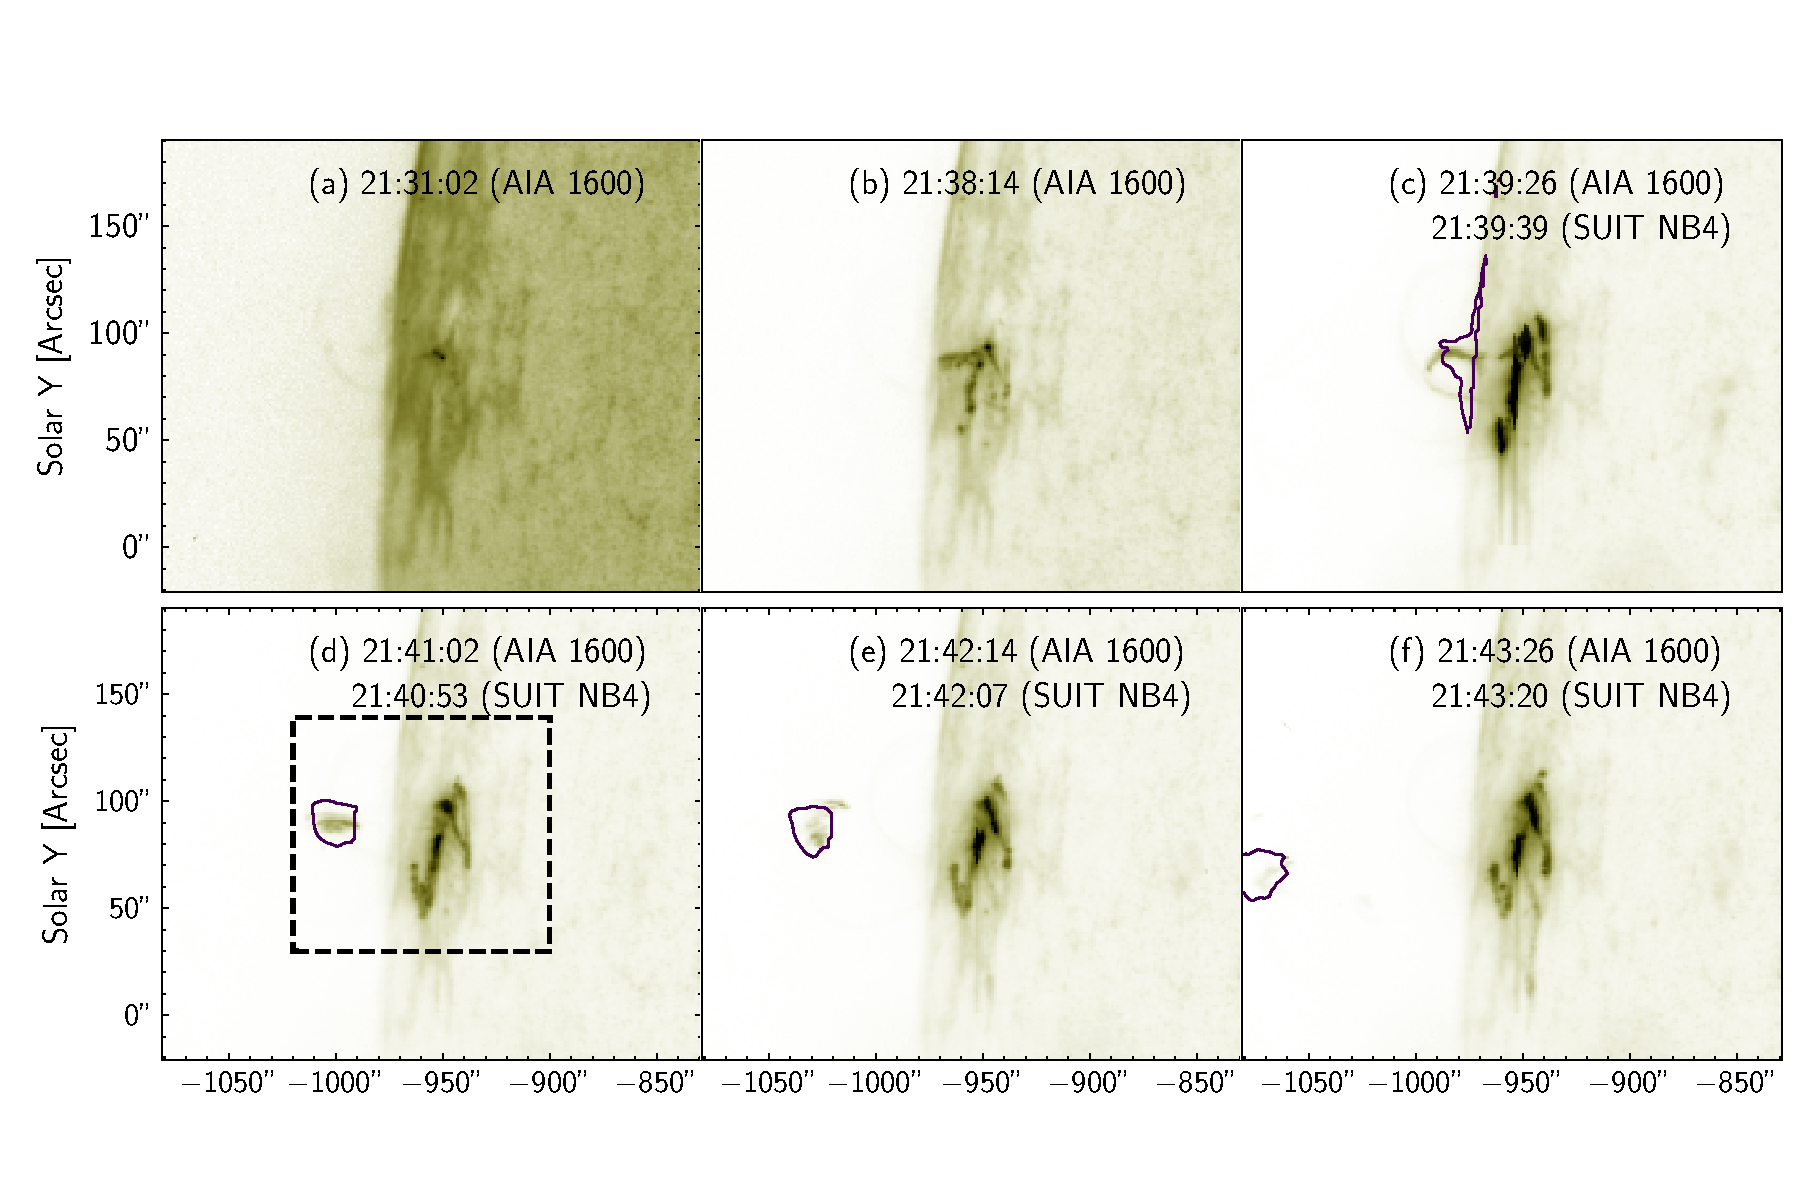
\includegraphics[trim = {0.5cm 0.7cm 0.2cm 2cm}, clip, width=0.7\linewidth]{fig1.pdf}
    \caption{Sequence of coaligned AIA 1600 {\AA} (black-green) and {\suit} NB4 (yellow) observations. We see the erupting loop and parts of the dense loops are co-spatial with the ejecta observed in {\suit} NB4 observations. An animated version of this sequence is available in the online version of the journal.}
    \label{fig:dec_flare_obs}
\end{figure*}
%%%%%%%%%%

We use DEMs calculated from AIA observations to investigate the thermal structure, using regularized inversion method described by \cite{hannah&kontar12}. We show the eruption in AIA 171 {\AA} inverted observation in Fig.~\ref{fig:dec_flare_dem}a. The red dashed box marked the region for the DEM analysis. In Fig.~\ref{fig:dec_flare_dem}b {--} g, we show the region from the red dashed box in various AIA cornal channels. Fig.~\ref{fig:dec_flare_dem}d shows AIA 171 {\AA} inverted (black) co-aligned with \suit~NB4 (yellow) observation. As illustrated earlier, the observed plasma blob in NB4 alignes with the brighter parts of the loop observed in various AIA channels. AIA channels with relatively hotter temperature response component, {\it i.e.} 94, 131, 193 {\AA} we see parts of the ejected loops which are not visible in colder channels, {\it i.e.} 171, 211, 335 {\AA}. In Fig.~\ref{fig:dec_flare_dem}h \& i, we show the emission measure (EM) and DEM weighted temperature of the region, calculated from the AIA observations. The 85\% intensity contour of the plasma blob observed in NB4 is marked with solid black line in Fig.~\ref{fig:dec_flare_dem}i. We mark a region on the same panel from the center of the ejected loop. We plot the DEMs from these two regions. We plot the calculated DEMs in Fig.~\ref{fig:dec_flare_dem}j, for the 85\% intensity contour (black circles) and the central part of the loop (red triangles) respectively. 

%%%%%%%%%%
\begin{figure*}[ht!]
    \centering
    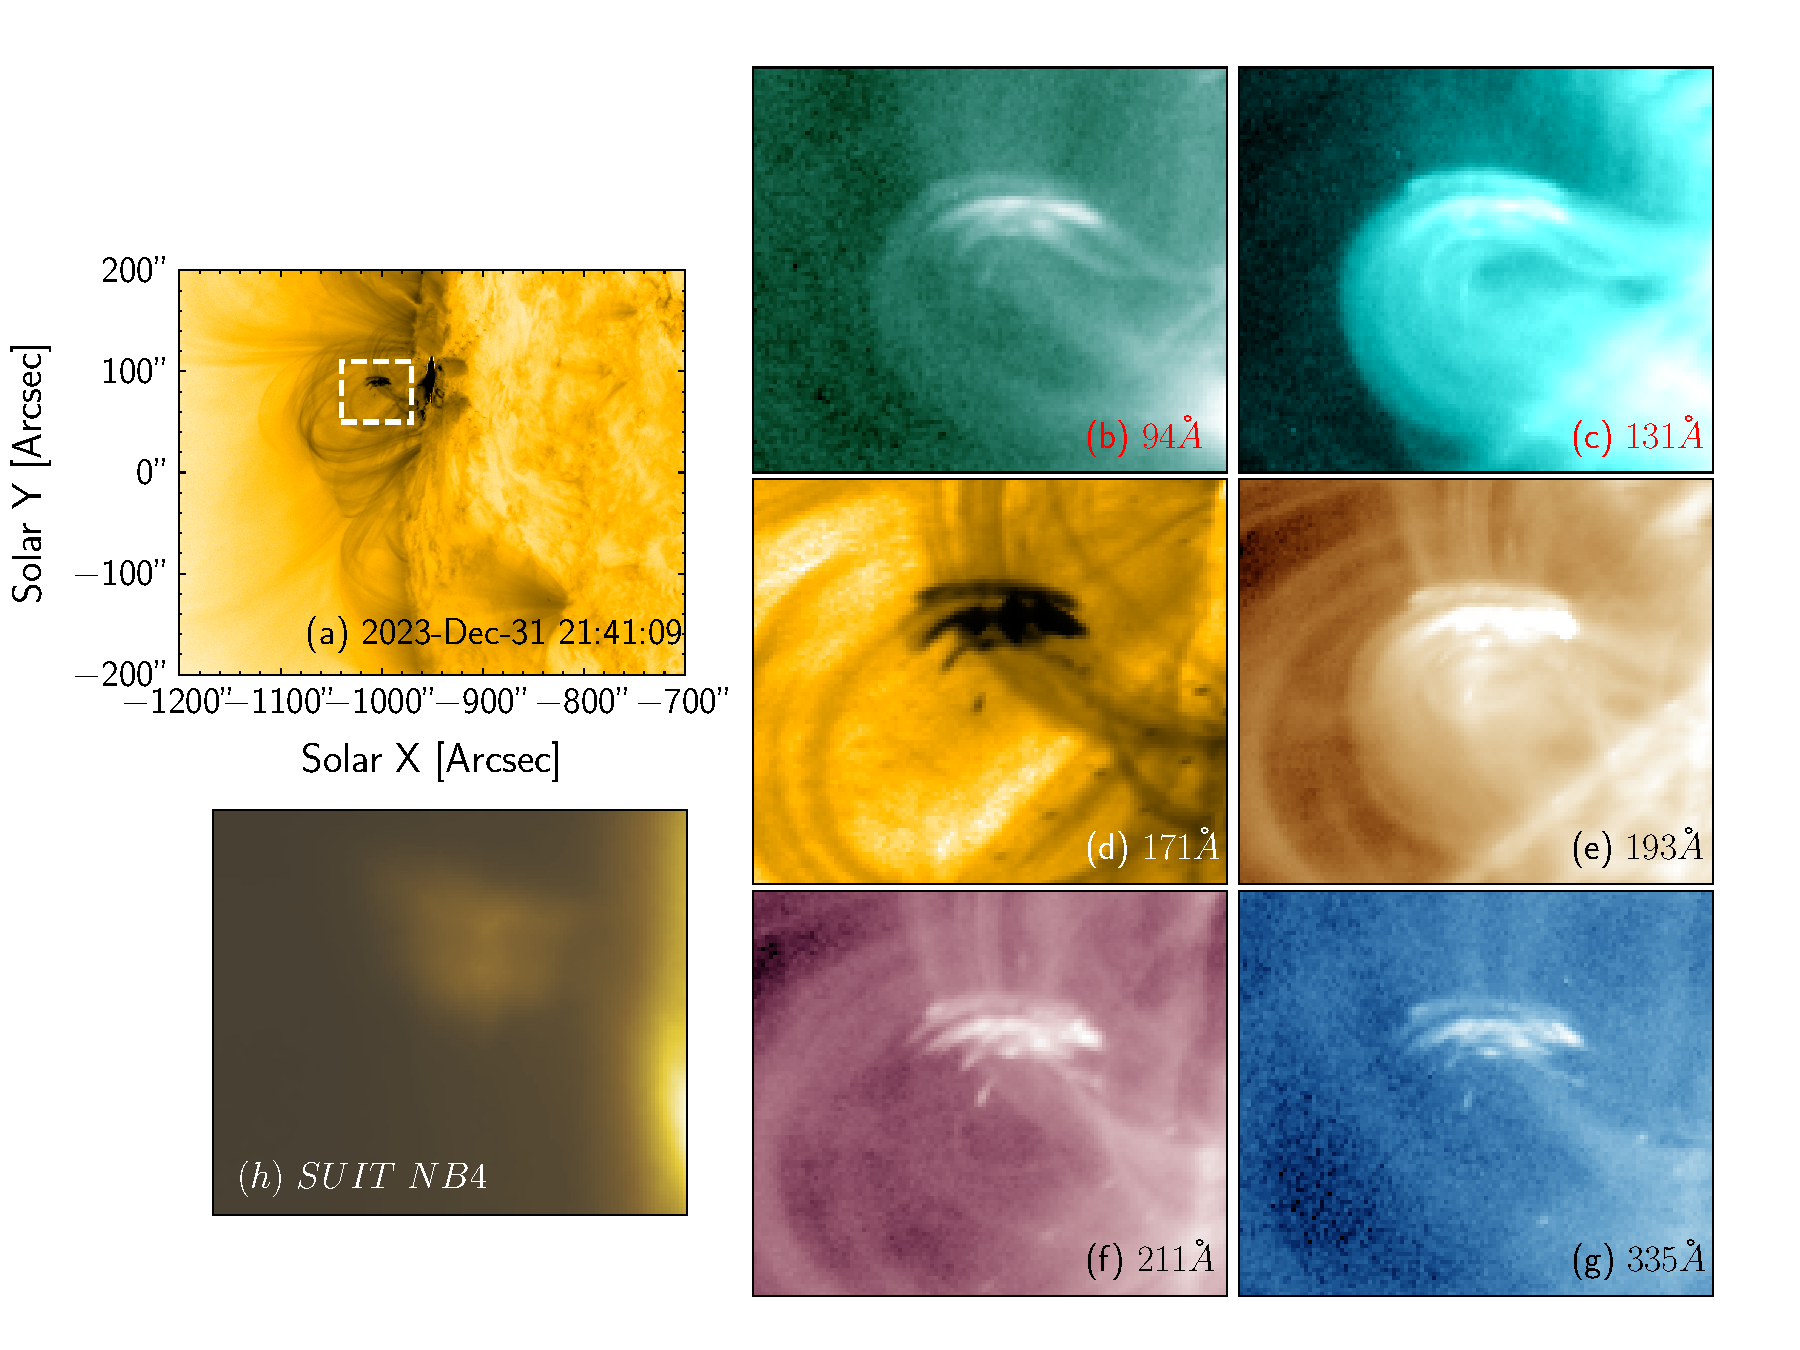
\includegraphics[trim = {1cm 0.5cm 3cm 0.5cm}, clip, width=0.7\linewidth]{fig2.pdf}
    \caption{(a) Inverted AIA 171 {\AA} observation during the ejection of the loop. Red dashed box marks the region considered for the DEM analysis. (b) {--} (g)  AIA observation in 94, 131, 171, 193, 211, and 335 {\AA} of the red dashed region respectively. The inverted 171 {\AA} observation (panel d) is overplotted on co-aligned \suit~NB4 observation (yellow). (h) Calculated EM from the AIA observations. (i) Calculated DEM weighted temperature from the AIA observations. The 85\% intensity contour of the \suit~NB4 blob is marked with solid black line. The dashed black line marks the central part of the loop. (j) The DEM from solid black contour and dashed black contour are plotted with black circles and red triangles respectively.}
    \label{fig:dec_flare_dem}
\end{figure*}
%%%%%%%%%%

We also calculate the velocity of the plasma blob from \suit~NB4 and AIA 1600 {\AA} observations and compare them. We show the trajectory of the plasma blob as observed from \suit~NB4 in Fig.~\ref{fig:dec_flare_dem}a. The position of the blob at various timestamp are marked with red cross. The velocity calculated bu tracing the ejecta is plotted in Fig.~\ref{fig:dec_flare_dem}b with blue circles (AIA 1600 {\AA}) and red triangles (\suit~NB4). The vertical dashed black line shows the start of the acceleration of the ejected material. Due to the larger field of view (FoV) of \suit~we can track the ejected material further out. In Fig.~\ref{fig:dec_flare_dem}c {--} f shows the sequence of observations from AIA 1600 {\AA} (purple) and 171 {\AA} (yellow-black). Fig.~\ref{fig:dec_flare_dem}g shows the {\it GOES} 1 {--} 8 {\AA} light curve during the flare. The four vertical red lines marks the times of Fig.~\ref{fig:dec_flare_dem}c {--} f. The soft X-ray flux reaches a plateau around 21:42 UT and starts to rise again after that, exhibiting multiple eruptions from the same active region.

%%%%%%%%%%
\begin{figure*}[ht!]
    \centering
    \includegraphics[trim = {0cm 1.7cm 0.5cm 2cm}, clip, width=0.7\linewidth]{fig3.pdf} \\
    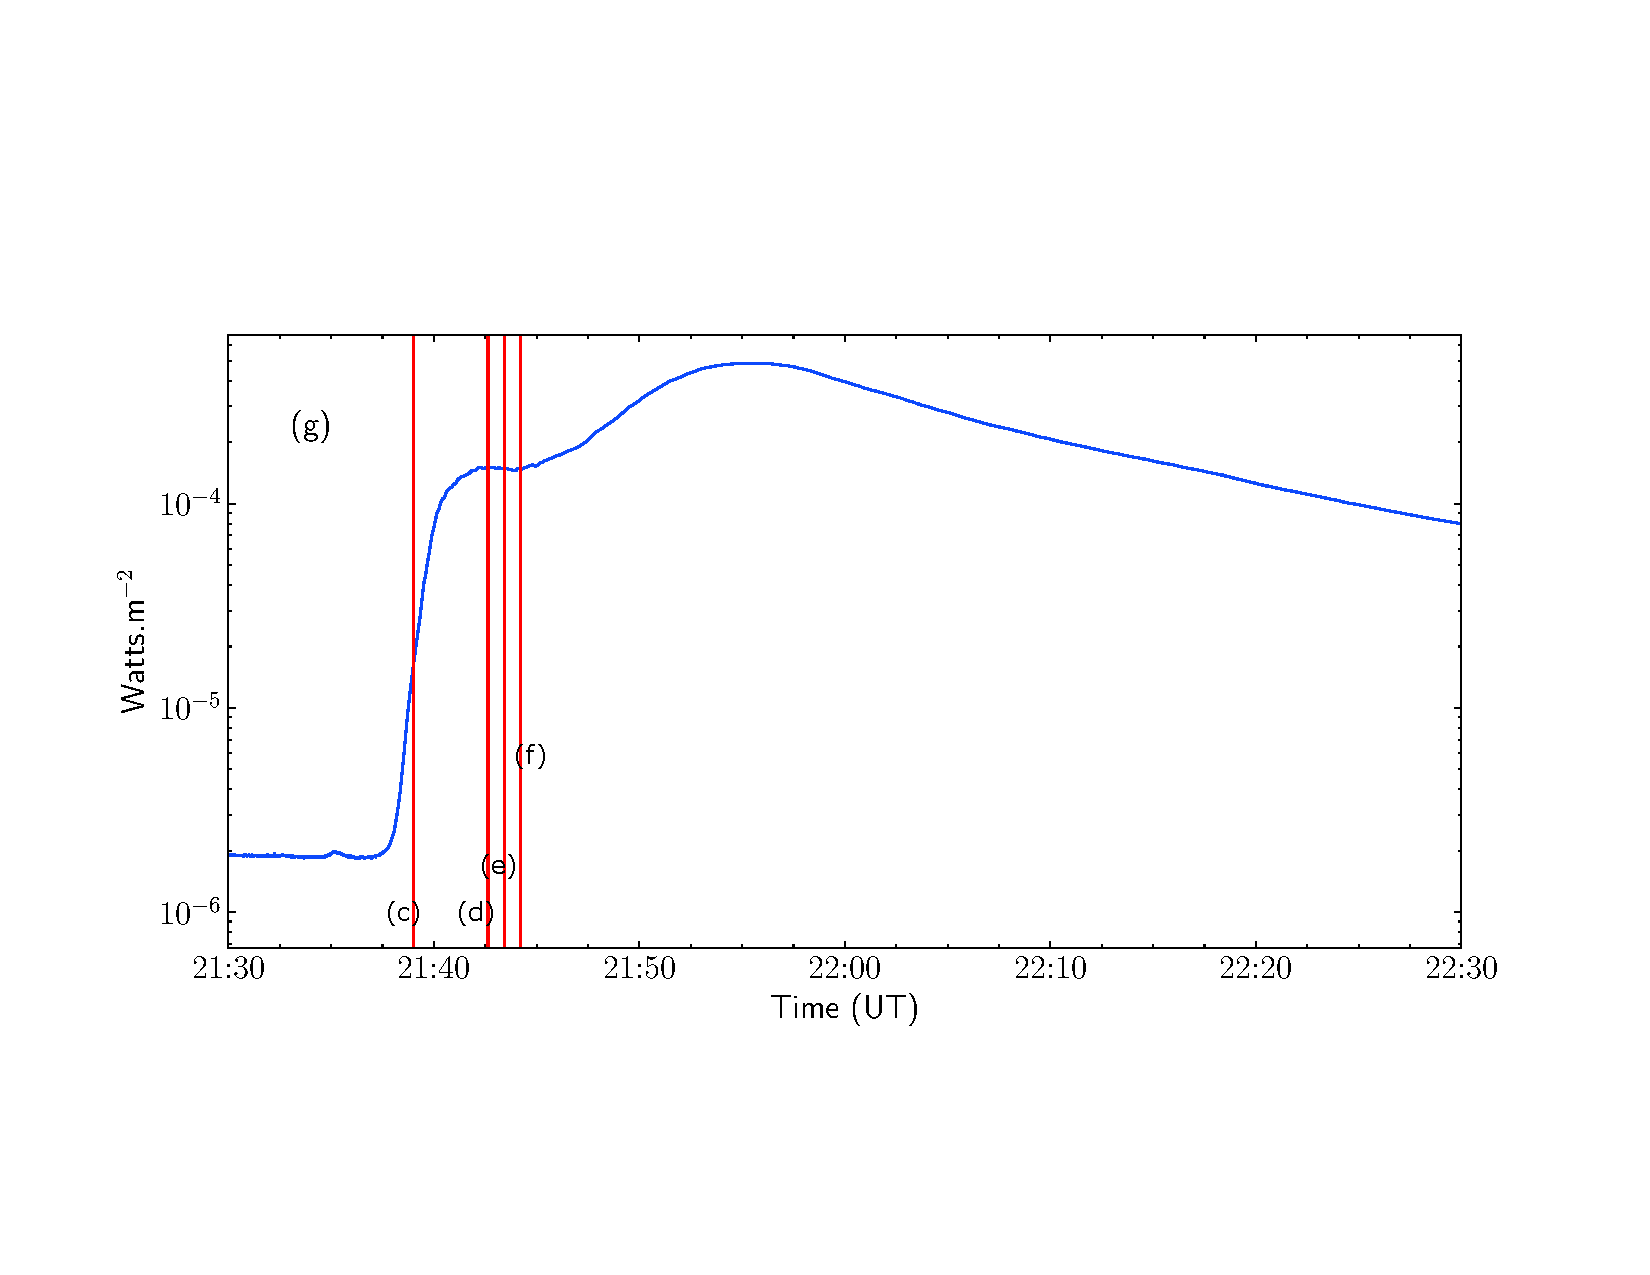
\includegraphics[trim = {1.5cm 4cm 2.5cm 5.5cm}, clip, width=0.5\linewidth]{fig3b.pdf} \\
    \caption{(a)\suit~NB4 observation at 21:42 UT. The trajectory of the plasma blob is marked with red crosses. (b) The velocity of the ejected material from AIA 1600 {\AA} (blue circle) and \suit~NB4 (red triangle) observation. The vertical dashed black line marks the start of acceleration. (c) {--} (f) Sequence of AIA 171 {\AA} inverted (yellow black) and 1600 {\AA} (purple) observations. A kink develops in the loops at 21:42 UT, marked with black arrow in (d). This is later ejected and accelerates. (g) GOES 1 {--} 8 {\AA} flux. The four vertical lines mark the times of panel (c) {--} (f).}
    \label{fig:dec_flare_vel}
\end{figure*}
%%%%%%%%%%

%%----------------------------------------------------
\subsection{Discussion} \label{sec:dec_31st_dis}
%%----------------------------------------------------

For the 31 December, 2023 X5 flare we only have (2k $\times$ 2k) one minute cadence observations in NB4 (\ion{Mg}{2} h). We see the eruption associated with the ejection of a plasma blob, which is cospatial with the ejected loops in AIA 1600 {\AA} and 171 {\AA}, as illustrated in Fig.~\ref{fig:dec_flare_obs}. We then investigate the thermal structure of the ejected loops from AIA observations, to understand the thermal environment of the plasma environment around the ejected material observed in NB4. From the AIA coronal channel observations, we find that parts of the ejected loop appear brighter and this bright region is cospatial with the ejected blob observed in NB4. From the DEM analysis we see that the central part of the ejected loop is hotter and less dense, compared to the parts of the loop which appear brighter (this is illustrated in Fig.~\ref{fig:dec_flare_dem}h \& i). In Fig.~\ref{fig:dec_flare_dem}i we mark the central part of the ejected loop with dotted black line and the 85\% intensity contour of the ejected NB4 plasma blob in black solid line. The DEM from these two regions are marked with red triangles and black circles respectively in Fig.~\ref{fig:dec_flare_dem}j. These DEMs clearly show that the region around the ejected material observed with NB4 have more colder material, resulting in overall colder DEM weighted temperature and denser surrounding environment.

%%%%%%%%%%%%%%%%%%%%%%
\begin{wrapfigure}{l}{0.45\textwidth}
    \centering
    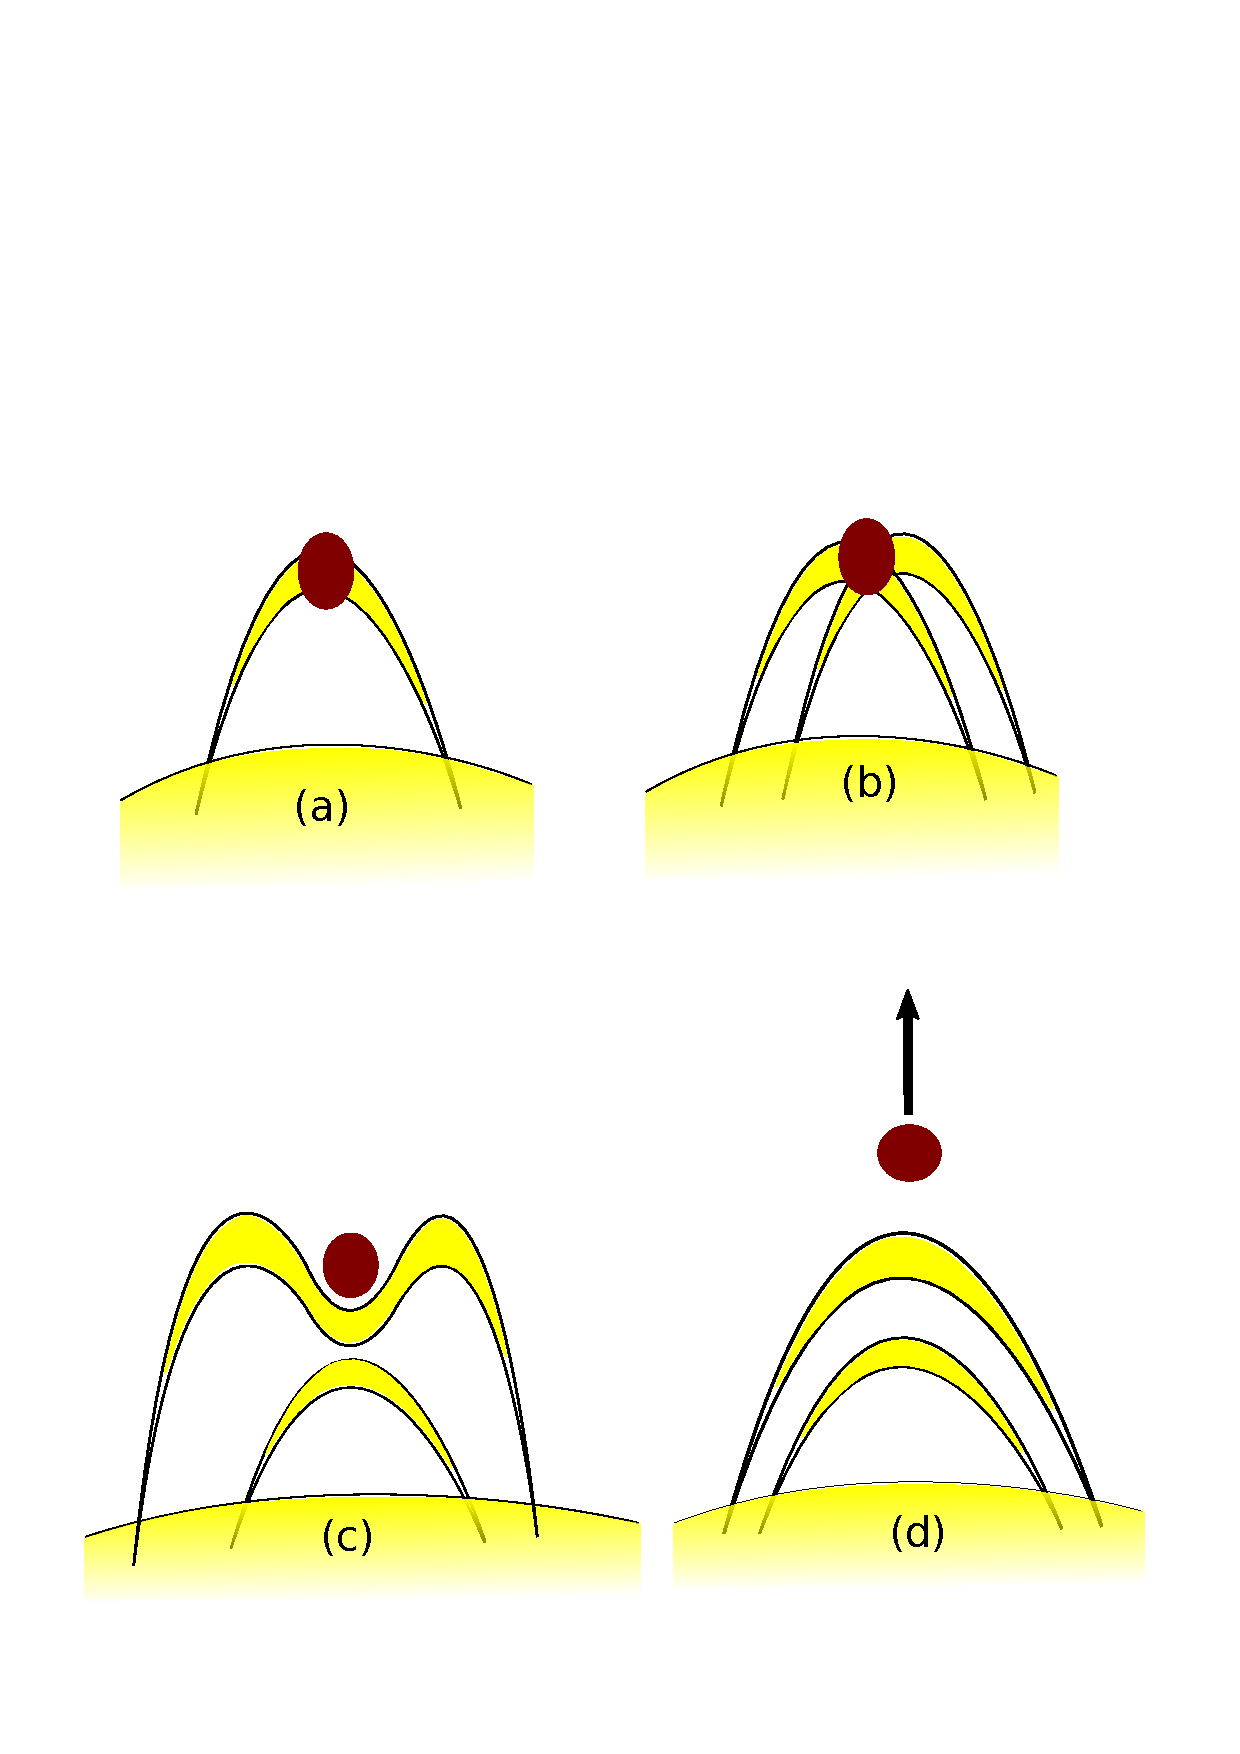
\includegraphics[trim={2cm 2.5cm 2cm 8.7cm}, clip, width=0.9\linewidth]{fig4.pdf}
    \caption{Sequence of cartoons depicting possible ejection mechanism for the cold plasma blob observed in {\suit} NB4.}
    \label{fig:cart}
\end{wrapfigure}
%%%%%%%%%%%%%%%%%%%%%%

We further investigate the kinematics of the ejected material. The ejection can be tracked further out with the {\suit} observations, albeit with much lower time cadence (1 minute) compared to AIA 1600 {\AA} (24 s). The velocity of the ejection is plotted in Fig.~\ref{fig:dec_flare_vel}b with blue circles (AIA 1600 {\AA}) and red triangles ({\suit} NB4). The measured velocities are consistent with each other. We see an acceleration at $\sim$ 21:42 UT. The tentative start of the acceleration is marked with a vertical dashed black line in Fig.~\ref{fig:dec_flare_vel}b. We see two successive eruption from the same active region wit the AIA observations. This is also illustrated by the {\it GOES} 1 {--} 8 {\AA} light curve in Fig.~\ref{fig:dec_flare_vel}g, as we see a first peak $\sim$ 21:40 UT and a second peak $\sim$ 21:55 UT. The two successive ejection is also consistent with the observed velocity structure. 

We show a possible mechanism to explain the ejection of the plasma blob in Fig.~\ref{fig:cart}. The initial eruption at $\sim$ 21:40 UT pushes cold dense material, as we see relatively steady rise from Fig.~\ref{fig:dec_flare_vel}b. Other loops from the same eruption, reconnects with the previous loops and develops a kink at $\sim$ 21:42 UT. The kink developing can be seen in Fig.~\ref{fig:dec_flare_vel}d, marked by black arrow. This is equivalent to the configuration in Fig.~\ref{fig:cart}c. The release of energy ejects the loop, as the acceleration is seen in the velocity profile after this in Fig.~\ref{fig:dec_flare_vel}b. This ejection is also accompanied by a subsequent brightening from the foot point as seen from AIA 1600 {\AA} observations in Fig.~\ref{fig:dec_flare_vel}e \& f. The SXR flux from this second eruption eventually peaks at $\sim$ 21:55 UT.

%%----------------------------------------------------
\section{X2.9 flare observed on May 27th, 2024} \label{sec:dec_31st}
%%----------------------------------------------------

NOAA AR 13697 was fully visible on the southeast limb from 29th May 2024. An X2.9 flare occurred from this active region on 27th May at 06:49 UT. The flare was localized by the onboard flare detection algorithm of {\suit} (For further details please refer to \citep{flare_det}). The event was located at $\sim$ [-920{\arcsec}, -250{\arcsec}] and the {\it GOES} SXR flux peaked at 07:08 UT. The footpoints of the flare were occulted behind the limb, ane the flare loops are only visible once they rise from behind the limb. 

Similar to the previous event we use the JPL horizons system to retrieve the position of Aditya-L1 and project the observations to Earth vantage. We then co-register and co-align AIA 1600 {\AA}, AIA 131 {\AA} and {\suit} NB4 observations. We show a sequence of co-aligned observations in Fig.~\ref{fig:may_flare_obs}. In Fig.~\ref{fig:may_flare_obs}a {--} c the {\suit} observations (yellow) are over-plotted on AIA 1600 {\AA} observations (green-black). This sequence shows the initial prominence eruption.

%%%%%%%%%%
\begin{figure*}[ht!]
    \centering
    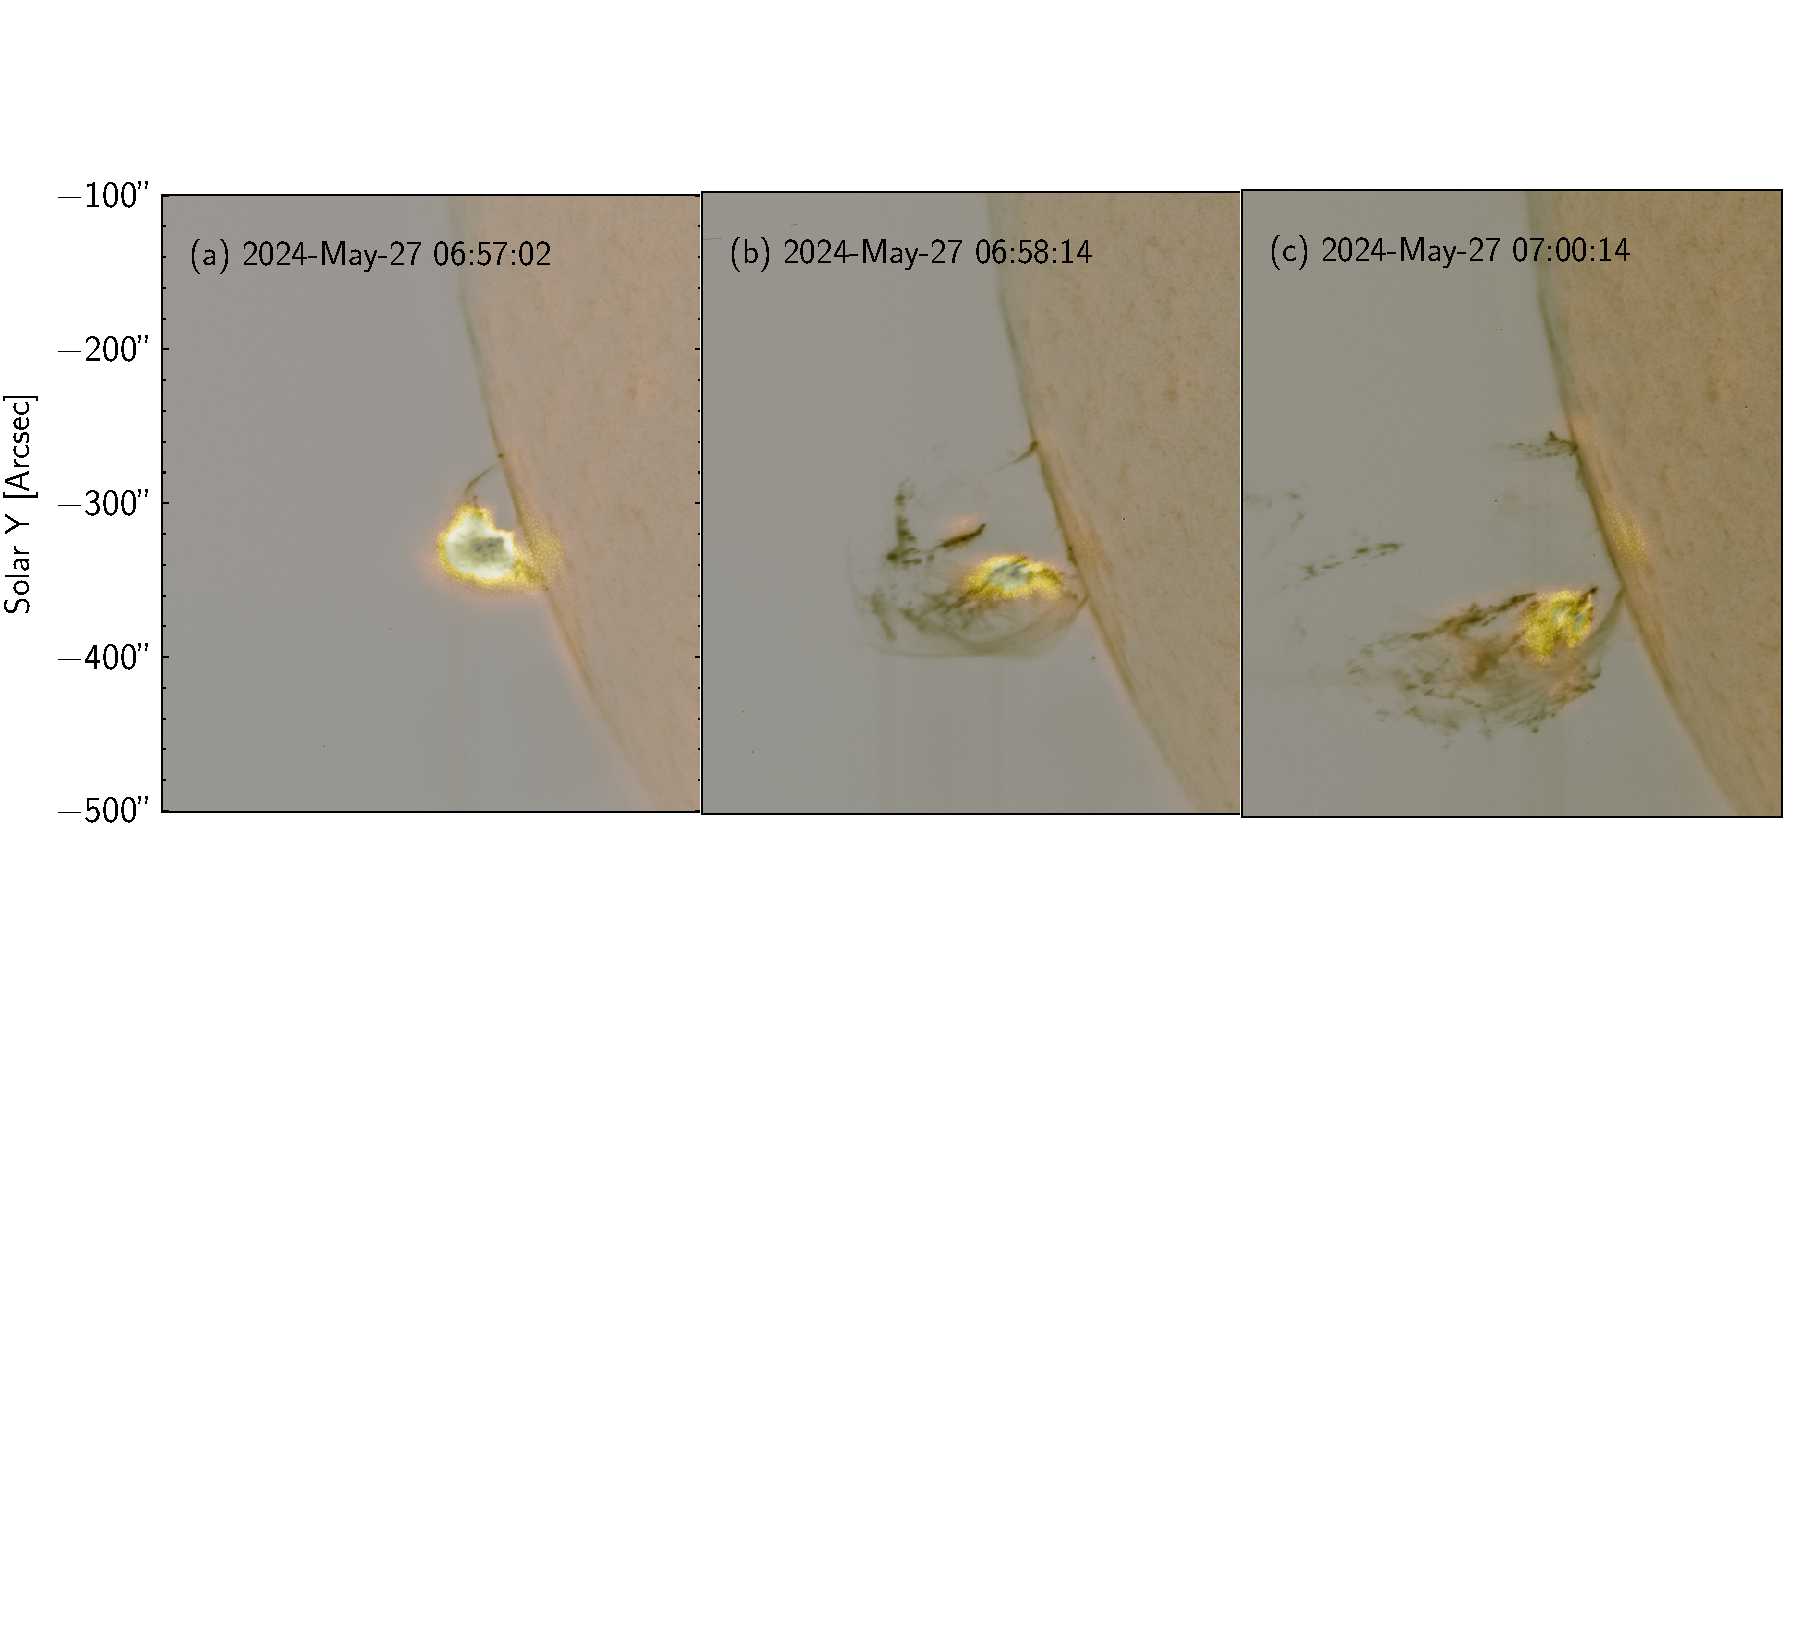
\includegraphics[trim = {0cm 0.7cm 0cm 2cm}, clip, width=0.7\linewidth]{fig1_.pdf}
    \caption{(a) {--} (c) Sequence of AIA 1600 {\AA} (black-green) observations coaligned with {\suit} NB3 (yellow) observations.}
    \label{fig:may_flare_obs}
\end{figure*}
%%%%%%%%%%

Similar to the previous event, we use DEMs calculated from AIA observations to investigate the thermal structure of the post flare loops. We show the post flare loops during the decay phase in Fig.~\ref{fig:may_flare_res}a. {\suit} NB4 (\ion{Mg}{2} h observation in yellow) is over-plotted on inverted AIA 131 {\AA} observation (blue-black). In Fig.~\ref{fig:may_flare_res}b \& c we plot the emission measure and DEM weighted temperature calculated from the AIA observations. The 80\% intensity contour of the off-limb {\suit} NB4 observations are marked in Fig.~\ref{fig:may_flare_res}c. 

%%%%%%%%
\begin{figure*}[ht!]
    \centering
    \includegraphics[trim={0.2cm 0cm 2cm 2cm}, clip, width=0.8\textwidth]{Figures/fig5.pdf}
    \caption{(a) AIA 131 {\AA} observation in inverted colormap (blue-black), coaligned with {\suit} NB3 observation (yellow). (b) Calculated emission measure from the AIA observation. (c) Calculated DEM weighted temperature from the AIA observation.}
    \label{fig:may_flare_res}
\end{figure*}
%%%%%%%%

%%%%%%%%%
\subsection{Discussion}\label{may27_dis}
%%%%%%%%%

Fig.~\ref{fig:may_flare_res}a we see that the {\suit} NB4 off limb features are cospatial wiht the base of the plasma sheet and top of the post flare arcades in AIA 131 {\AA} observations (blue-black). We mark the 85\% intensity contour of {\suit} NB4 observation in the subsequent panels b \& c, which show the emission measure and DEM-weighted temperature calculated from the AIA observations.

The {\suit} NB4 observations are co-spatial with low temperature and relatively low-density region at the loop top, just below the plasma sheet. There is a higher-density region right on top of this region at the base of the plasma sheet. Please note that the density and temperature calculated here are calculated from AIA observations, which are not as sensitive to plasma outside of $\log \mathrm{T} \sim$ 5 {--} 7.5 K. The low density at the loop top can easily be attributed to the plasma being outside of this temperature range. But that would be in contradiction to one of the standard scenarios of post-flare loops, where it is assumed that the post-flare loop-top brightening is created by a collision of evaporating flows from the foot-points and results in elevated density and temperature at the loop top. This has also been demonstrated from 1d loop simulations \citep{sharma16, reeves07}.

%%%%%%%%%%%%
\section{Outlook}
%%%%%%%%%%%%